% Options for packages loaded elsewhere
\PassOptionsToPackage{unicode}{hyperref}
\PassOptionsToPackage{hyphens}{url}
\documentclass[
]{article}
\usepackage{xcolor}
\usepackage[normalem]{ulem} % \sout is available, but can be fragile in technical text
\newcommand{\rev}[1]{\textcolor{blue}{#1}}

% Change-tracking helpers
% IMPORTANT: do NOT wrap environments (equation/align/figure/...) in these macros.
% Keep deletions visible but robust (no \sout) to avoid runaway arguments.
\newcommand{\revdel}[1]{\textcolor{red}{#1}}
\newcommand{\revred}[1]{\textcolor{red}{#1}}
\newcommand{\revgreen}[1]{\textcolor{green!50!black}{#1}}
\newcommand{\revpurple}[1]{\textcolor{violet}{#1}}
\newcommand{\revpurpdel}[1]{\textcolor{violet}{#1}}

% For deleted displayed equations: keep the equation valid LaTeX, but color it.
\newenvironment{revpurpdelequation}{\begingroup\color{violet}\begin{equation}}{\end{equation}\endgroup}

% For multi-paragraph revision blocks (\textcolor can’t handle paragraph breaks).
\newenvironment{revbrownblock}{\begingroup\color{brown}}{\endgroup}

\newcommand{\revorange}[1]{\textcolor{orange}{#1}}
\newcommand{\revpink}[1]{\textcolor{magenta}{#1}}
\newcommand{\revturquoise}[1]{\textcolor{teal}{#1}}
\newcommand{\revbrown}[1]{\textcolor{brown}{#1}}
\usepackage{amsmath,amssymb}
\usepackage[european]{circuitikz}
\setcounter{secnumdepth}{-\maxdimen} % remove section numbering
\usepackage{iftex}
\ifPDFTeX
  \usepackage[T1]{fontenc}
  \usepackage[utf8]{inputenc}
  \usepackage{textcomp} % provide euro and other symbols
\else % if luatex or xetex
  \usepackage{unicode-math} % this also loads fontspec
  \defaultfontfeatures{Scale=MatchLowercase}
  \defaultfontfeatures[\rmfamily]{Ligatures=TeX,Scale=1}
\fi
\usepackage{lmodern}
\ifPDFTeX\else
  % xetex/luatex font selection
\fi
% Use upquote if available, for straight quotes in verbatim environments
\IfFileExists{upquote.sty}{\usepackage{upquote}}{}
\IfFileExists{microtype.sty}{% use microtype if available
  \usepackage[]{microtype}
  \UseMicrotypeSet[protrusion]{basicmath} % disable protrusion for tt fonts
}{}
\makeatletter
\@ifundefined{KOMAClassName}{% if non-KOMA class
  \IfFileExists{parskip.sty}{%
    \usepackage{parskip}
  }{% else
    \setlength{\parindent}{0pt}
    \setlength{\parskip}{6pt plus 2pt minus 1pt}}
}{% if KOMA class
  \KOMAoptions{parskip=half}}
\makeatother
\usepackage{graphicx}
\setkeys{Gin}{width=\linewidth,keepaspectratio}
\makeatletter
\newsavebox\pandoc@box
\newcommand*\pandocbounded[1]{% scales image to fit in text height/width
  \sbox\pandoc@box{#1}%
  \Gscale@div\@tempa{\textheight}{\dimexpr\ht\pandoc@box+\dp\pandoc@box\relax}%
  \Gscale@div\@tempb{\linewidth}{\wd\pandoc@box}%
  \ifdim\@tempb\p@<\@tempa\p@\let\@tempa\@tempb\fi% select the smaller of both
  \ifdim\@tempa\p@<\p@\scalebox{\@tempa}{\usebox\pandoc@box}%
  \else\usebox{\pandoc@box}%
  \fi%
}
% Set default figure placement to htbp
\def\fps@figure{htbp}
\makeatother
\setlength{\emergencystretch}{3em} % prevent overfull lines
\providecommand{\tightlist}{%
  \setlength{\itemsep}{0pt}\setlength{\parskip}{0pt}}
\usepackage{bookmark}
\IfFileExists{xurl.sty}{\usepackage{xurl}}{} % add URL line breaks if available
\urlstyle{same}
\hypersetup{
  pdftitle={\rev{Electromagnetic Simulation of Pilot Tone Signal Modulation During Cardiac Motion}},
  hidelinks,
  pdfcreator={LaTeX via pandoc}}

\title{\rev{Electromagnetic Simulation of Pilot Tone Signal Modulation During Cardiac Motion}}
\author{}
\date{}

\usepackage[backend=biber, style=numeric, sorting=none]{biblatex}
\addbibresource{references.bib} % Mit .bib am Ende!

\begin{document}
\maketitle

\textbf{Authors:}

Mario Bacher\textsuperscript{1,2}

Matthias Stuber\textsuperscript{2,3}

Peter Speier\textsuperscript{1}

\textbf{Affiliations:}

\textsuperscript{1} Siemens Healthineers AG, Erlangen, Germany

\textsuperscript{2} Department of Diagnostic and Interventional
Radiology, Lausanne University Hospital (CHUV) and University of
Lausanne (UNIL), Lausanne, Switzerland

\textsuperscript{3} Center for Biomedical Imaging (CIBM), Lausanne,
Switzerland

\textbf{Corresponding Author:}

Mario Bacher

Siemens Healthineers AG

SHS DI MR R\&D SWI CFP

Allee am Roethelheimpark 2

91052 Erlangen

Germany

mario.bacher@siemens-healthineers.com

\section{Abstract}\label{abstract}

\subsection{Purpose}\label{purpose}

The Pilot Tone (PT) navigator is a novel electromagnetic motion sensor
that enables contactless respiratory and cardiac motion sensing for
clinical MRI. Here, we aim to present \rev{the first full-wave electromagnetic simulation framework for investigating} the
physical processes underlying the Pilot Tone navigator \rev{using a realistic digital human phantom}.

\subsection{Methods}\label{methods}

We performed electromagnetic simulations on a realistic digital human
phantom capable of simulating cardiac motion. We demonstrate in-silico
how the induction of eddy currents in conductive tissues leads to the
generation of a secondary magnetic field which can be sensed by coil
arrays, specifically by the receive subsystem of commercial MRI system.
We further show how the received signal modulation is distributed
spatially in the scan volume.

\subsection{Results}\label{results}

Differences in conductivity between tissues and their movement during
the cardiac cycle is the driving force behind the observed PT signal
modulation. Simulations \rev{reproduce expected signal modulation trends and provide mechanistic insight into} how signal modulation due to
cardiac motion can be sensed throughout the measurement volume. The
measured signal modulation is \revred{quantitatively} strongly correlated to total cardiac
volume \revred{($|R| > 0.94$)}.

\subsection{Conclusion}\label{conclusion}

\rev{Our simulation framework demonstrates how inductive coupling via
conductive tissues shapes the PT signal and provides mechanistic understanding of the modulation process.}

The complex amplitude and phase modulation patterns generated by tissue
motion in the multi-coil data makes PT navigators an attractive
technique for measuring physiological motion independently of sequence
parameters and trajectory while being both easy to use and requiring no
patient preparation.

Keywords\textbf{:} Pilot Tone, cardiac and respiratory motion,
electromagnetic motion sensor, FDTD, navigator

\section{Introduction}\label{introduction}

The Pilot Tone (PT) navigator, proposed by Speier et al. \cite{Speier2015PT-Nav:MR-receiver} is a
novel, contactless method of sensing both cardiac and respiratory motion
in real-time for clinical MRI systems without the need for ECG
electrodes, pulse oximetry devices, navigators, or respiratory bellows.
This method is based on a weak continuous high frequency radiofrequency
signal \cite{NationalCommunicationsSystemTechnologyStandardsDivision1996} emitted into the bore, can be easily integrated in
current-gen commercial MRI scanners, requiring only a simple RF
generator and transmit loop. This signal is then modulated by
physiological motion and received using the existing MR receiver
hardware.

While Pilot Tone navigation has been used successfully by several groups
for respiratory \cite{Vahle2020RespiratoryTone, Rigie2018TrackingNavigation, Koesters2016MotionNavigators, Lenk2018RespiratoryTechnology, Schroeder2016a, Anand2021BeatNavigators}, cardiac \cite{BacherPilotInitialization, Bacher2018PilotCine, Bacher2017RetrospectiveCohort, Bacher2017CardiacStudy, BacherPerformanceFramework, Schroeder2016} and combined respiratory
and cardiac triggering and gating \cite{Falcao5DGating, BacherRetrospectiveCohort}, the underlying physics
have not yet been thoroughly investigated. In this work we aim to
provide a theoretical foundation for this novel method. We then use
numerical electromagnetic simulations to visualize and investigate the
physical processes underlying the Pilot Tone navigator.

Contactless motion sensing techniques based on modulation of
electromagnetic parameters due to physiological motion have been under
\cite{Moskalenko1960, Moskalenko1958}
demonstrated the modulation of high-frequency radio wave transmission
and reflection by physiological motion such as blood-flow and
respiratory volume changes. Guy et al. \cite{Johnson1972} expanded on the idea and
demonstrated that variation in transmission loss of a 915MHz microwave
beam passing through the human chest is proportional to ventricular
volume changes in the heart. At microwave frequencies, transmission loss
and reflection (similar to radar) can be measured \cite{MatsumotoHeartbeatAnalysis, Pfanner2014, Pfanner2013}. At lower
frequencies, modulation of inductive coupling can be used to detect
motion. Tarjan and McPhee {\cite{Tarjan1968ElectrodelessInduction} first demonstrated sensing of
respiratory and cardiac motion in two inductively coupled coils at
100kHz. The underlying principle of measuring an objects resistivity via
eddy currents generated in the object has been used extensively in a
wide array of fields since the early 20\textsuperscript{th} century such
as geophysics \cite{Slichter1933TheStructures, Everett2012TheoreticalSurface}, oceanography \cite{Striggow1985TheApplication}, non-destructive
testing in the process industry \cite{Garcia-Martin2011Non-destructiveTesting, Sureshkumar2013UtilizationFBRs, Kumar2016TowardsModel} and, in a medical context in
magnetic induction tomography (MIT) to image electromagnetic tissue
properties \cite{Griffiths1999MagneticTissues}.

In recent years, electromagnetic motion sensing has become an active
field of research driven by the availability of cheap, easy to use
transmit-receive systems based mostly on Wi-Fi \cite{Liu2016ContactlessDevices, Yang2018Multi-personDevices} and RFID
\cite{Hui2018MonitoringSensing, Liu2019VitalChallenges}, often in the form of wearable sensors \cite{Teichmann2014TheArray, Teichmann2010RespirationCoil} or
embedded in furniture such as patient beds \cite{Mahdavi2017In-bedGradiometer}.

In the MR community, three methods based on electromagnetic interactions
with tissue have been proposed recently. These can be roughly classified
into active methods where the modulation of some external reference
signal is measured and passive methods that do not use an external
reference. The basis for all these methods is that biological tissues
have different dielectric properties: permittivity and conductivity. The
spatial distribution of tissue thus governs the observed impedance and
any motion that changes this spatial distribution may lead to a change
in the observed impedance.

Andreychenko et al. \cite{Andreychenko2017ThermalSensor, Navest2019UnderstandingNavigator} use the thermal noise variance ,
measured in the bandwidth in the oversampling (at least twofold, to
ensure the used bandwith does not contain image information) for
monitoring: At frequencies \textgreater27MHz, the real part of the MR
scanners receive coil impedance is dominated by body resistance and thus
any motion that effectively alters body impedance modulates thermal
noise variance \cite{Andreychenko2017ThermalSensor}. Since noise is measured directly, without an
external reference, we classify this noise navigator as a passive
method.

Buikman et al. \cite{Buikman1988TheImaging} use reflected power in the transmit path due to
impedance mismatch of a transmit body coil to detect motion. Jaeschke et
al. \cite{Jaeschke2018Cardiac7T, Jaeschke2017, Jaeschke2017a, Jaeschke2019ScatteringMonitoring} expanded on this method by measuring the scattering
matrix in a parallel transmit array, which describes the reflection
between the channels of a parallel-transmit (pTx) system. The Tx pulse
itself acts as the reference signal, making this an active method by our
classification. When the imaging RF pulse is combined with a
simultaneous S-matrix measurement pulse that is unique for each channel,
it is possible to effectively use as many separate reference signals as
transmit elements.

A prime advantage of the methods described above as well as Pilot Tone
is the relatively simple integration in current generation MRI systems
without the need for complex additional hardware. However, due to the
use of the scanners receive system, the used frequency is constrained to
frequencies close to the Larmor frequency.

Anand and Lustig \cite{Anand2021BeatNavigators, Anand2024BeatFrequencies} recently proposed a method where the
single carrier wave with a frequency close to the Larmor frequency is
replaced by two waves with two different frequencies in the low GHz
range such that a motion-modulated standing wave pattern is created. The
two frequencies are deliberately chosen such that their modulation
product, created by intermodulation in the receive chain, falls into the
receivers useable bandwidth.

In contrast, our proposed Pilot Tone navigator uses a single, continuous
wave external reference signal, making it an active method. The
reference signal or ``Pilot Tone'' is transmitted via a small loop-coil
positioned anterior to the chest wall, in close proximity to the
subject's heart.

While this method could be implemented in any imaging modality, MRI is
an especially attractive platform as the necessary high-end receiver
hardware already exists.

Consequently, the Pilot Tone frequency \(f_{PT}\) is chosen such that it
lies within the receiver's operating bandwidth but has enough separation
in the frequency domain to the bandwidth occupied by the MR signal to
not interfere with imaging.

\rev{In practice, the PT signal is separated from the MR imaging signal in the frequency domain. The PT amplitude and phase are extracted from a narrow spectral bin centered at $f_{PT}$ in the digitized receiver data. The present work models only the electromagnetic physics of the modulation mechanism; the signal processing aspects of PT extraction are beyond its scope.}

Since most biological tissues are almost completely transparent to
magnetic fields, having relative permeabilities
\(\mu_{r,tissue} = 1 + \chi_{tissue} \approx 1\)
\(,\ because\ the\ range\ for\ human\ tissues\ is\ only\ \chi_{tissue} \approx ( - 11\ \ldots\  - 7) \times 10^{- 6}\)
\cite{HasgallITISTissues}, the generated magnetic field penetrates the subject's body
almost unchanged. Most tissues however are conductive and therefore the
continuous wave magnetic field induces eddy currents. These eddy
currents then in turn create a secondary magnetic field which is
superimposed to the excitation (primary) field, leading to modulations
of the magnetic field received in the receive coil.

Having previously demonstrated \cite{Vahle2020RespiratoryTone, Bacher2018PilotCine, BacherRetrospectiveCohortb, Bacher2017CardiacStudy} the feasibility of using
Pilot Tone as a replacement for ECG and respiratory belts or navigators
in practical applications, both retrospective and real-time, we now aim
to provide a theoretical foundation to the method. We outline how the
received signal modulation can be explained by Maxwell's equations and
then use numerical simulations to perform virtual experiments. The Pilot
Tone navigator has so far been implemented on 1.5T and 3T systems and
has been found to compare favorably to ECG triggering. \cite{Bacher2020PerformanceFramework, Qian2025ComparisonStudy, Mizuno2024ClinicalLeads}

\section{Theory}\label{theory}

To better understand the underlying physical mechanisms of the Pilot
Tone, we first focus on the simplest case of one signal-generating coil
\(L_{G}\) and one receiving coil \(L_{R}\) as depicted in Figure~\ref{fig:coupling-model}a. The
generating coil \(L_{G}\) is excited by a continuous harmonic current
\(i_{G}(t)\) with frequency \(f_{PT}\), the receiving coil \(L_{R}\) is
connected to an ideal measurement circuit and positioned at a distance
\(d_{GR}\) from \(L_{G}\). Both coils are surrounded by a magnetically
and electrically non-conductive medium (vacuum, air).~

Applying the current \(i_{G}\) gives rise to a time-varying magnetic
field \(\mathbf{B}_{G}\) around \(L_{G}\). The magnetic flux
\(\Phi_{G}\) through the area encompassed by the receiving coil
\(L_{R}\) then induces an electromotive force \(\varepsilon\) in
\(L_{G}\):

\begin{equation}
\label{eq:flux}
\Phi_{G} = \int_{\Sigma}\mathbf{B}_{G} \cdot d\mathbf{A}
\end{equation}

\begin{equation}
\label{eq:faraday}
\varepsilon = -\frac{d\Phi_{G}}{dt}
\end{equation}

where \(\mathbf{B}_{G} \cdot d\mathbf{A}\) in Eq.~\eqref{eq:flux} is an infinitesimal amount
of magnetic flux in the receiving element. The induced current flows in
the direction that opposes the charge which produced it (Lenz's law).

The ideal measurement circuit connected to \(L_{R}\) will thus measure
an AC voltage of the same frequency as \(f_{PT}\) with amplitude and
phase determined by the geometry, i.e. distance and angle of the area
\(A\) with respect to \(\mathbf{B}_{G}\).

\subsection{Generator loop
characteristics}\label{generator-loop-characteristics}

Without loss of generality, we construct the generating coil \(L_{G}\)
as a single loop and feed it with input power of \(0dB_{m}\). In
practice, when faced with the challenge of integrating this loop into an
MR coil array, special care must be taken to minimize direct inductive
coupling to neighboring Rx elements. This can be done by geometric
decoupling, i.e. deliberate choice of coil overlap by positioning and
choosing more complex shapes for the loop geometry. Note that in any
case the geometric dimensions, especially the length of \(L_{G}\) is
very small compared to the wavelength \(\lambda\) at the used
frequencies.

This has two important implications: First, the distances between the
generating coil and the receiving coil(s) must be much smaller than the
wavelength in air: We then operate in the ``near-field'', a volume
around an antenna-like structure, typically defined as
\(r < \frac{\lambda}{2\pi}\), where the electric and magnetic field can
be seen as independent and no EM-wave forms. By this definition, the
near-field at the Pilot Tone frequencies chosen by us at typical
clinical field strengths of 1.5T and 3T extends to r=0.76m at 62.5MHz
(1.5T) and r=0.39m at 122.5MHz (3T) in vacuum/air.


\revorange{It is important to note that the near-field condition is not merely a simplification adopted in this work but a consequence of the system design and bore geometry. In our PT implementation, the carrier frequency was constrained to lie just outside the MR imaging band so that the signal could be received by the existing MR receive chain. At 1.5T and 3T this places the PT frequency at 62.5\,MHz and 122.5\,MHz respectively, well within the near-field regime.}

\revorange{Furthermore, the MRI bore itself enforces this condition: the bore liner is a conductive metal cylinder that acts as a circular waveguide \textcolor{red}{\cite{Brunner2009TravellingWave, Tang2011CutoffFree}}. The dominant TE\textsubscript{11} mode has a cutoff frequency of $f_c = \chi'_{11} c / (2\pi a)$, where $\chi'_{11} = 1.8412$ is the first zero of the Bessel function derivative and $a$ is the bore radius \textcolor{red}{\cite{Pozar2012Microwave}}. For a 70\,cm bore ($a = 0.35$\,m), $f_c \approx 251$\,MHz, well above both PT frequencies. Below cutoff, electromagnetic fields cannot propagate along the bore axis. They are evanescent and decay exponentially as $e^{-\alpha z}$ with attenuation constants of $\alpha \approx 44$\,dB/m at 62.5\,MHz and $\alpha \approx 40$\,dB/m at 122.5\,MHz.}

\revorange{Consequently, even when the PT generator is placed on the bore wall or farther from the patient rather than directly on the body, the coupling remains reactive (near-field) in nature, not radiative. The bore suppresses far-field propagation, and all coupling occurs through evanescent modes. This explains why practical PT implementations with generators at various positions along the bore, including configurations that appear to violate the free-space near-field distance criterion $r < \lambda / 2\pi$, still produce usable motion signals \textcolor{red}{\cite{Vahle2020RespiratoryTone, Rigie2018TrackingNavigation}}. In contrast, Anand and Lustig \textcolor{red}{\cite{Anand2024BPT}} recently demonstrated that carrier frequencies above the bore cutoff (1.2--2.4\,GHz) enable propagating waveguide modes with fundamentally different, frequency-dependent motion sensitivity.}

Secondly, the length of \(L_{G}\) is much smaller than the wavelength,
thus \(L_{G}\) is an ``electrically-small'' antenna in which the
generated magnetic field dominates, and the generated electric field can
be neglected \cite{Bolton2020OptimalAntenna}. Electric fields are however still generated in
the body, giving rise to displacement currents which are a contributor
to the magnetic field generated by eddy currents. \revpurple{A quantitative analysis showing that the Faraday-induced electric field in the body dominates over the loop-generated electric field by an order of magnitude is provided in Appendix~\ref{app:derivation}.}

\subsection{Conductive regions}\label{conductive-regions}

Consider now a conductive domain \(\Gamma_{\sigma 1 > 0}\) placed in
proximity to \(L_{G}\) and \(L_{R}\) (Figure~\ref{fig:coupling-model}a) such that it intersects
the field-lines generated by \(L_{G}\): The magnetic field
\(\mathbf{B}_{G}\) now induces an electromotive force in
\(\Gamma_{\sigma 1 > 0}\), forming eddy-currents which in turn create a
secondary magnetic field \(\Delta\mathbf{B}\) (Figure~\ref{fig:coupling-model}b). The
Maxwell-Faraday equation

\begin{equation}
\label{eq:maxwell-faraday-tissue}
\nabla \times \mathbf{E}_{\text{tissue}} = -\frac{\partial \mathbf{B}_{G}}{\partial t}
\end{equation}

states that a time- and/or spatially varying magnetic field always
accompanies a time- and/or spatially varying electric field and vice
versa. \revpurpdel{This secondary magnetic field \(\mathbf{H}_{\mathbf{e}}\) created
in the eddy-current region \(\Gamma_{\sigma 1 > 0}\) can be expressed by
Ampere's circuital law with Maxwell's addition (considering the
displacement current) in the macroscopic formulation, i.e. with matter
present}

\begin{revpurpdelequation}
\nabla \times \mathbf{B}_{e}
= \mu_{0}\left(\mathbf{J}_{\text{tissue}} + \frac{\partial \mathbf{D}_{\text{tissue}}}{\partial t}\right)
= \mu_{0}\left(-\sigma_{\text{tissue}}\frac{\partial \mathbf{B}_{G}}{\partial t} + \varepsilon_{\text{tissue}}\frac{\partial^{2} \mathbf{B}_{G}}{\partial t^{2}}\right)
\end{revpurpdelequation}

\revpurple{The induced current density in the tissue is $\mathbf{J}_{\text{tissue}} = \gamma\,\mathbf{E}_{\text{tissue}}$, where $\gamma = \sigma + j\omega\varepsilon$ is the complex admittivity combining conductivity $\sigma$ and permittivity $\varepsilon$. As all biological tissues are non-magnetic ($\mu \approx \mu_0$), the permeability of vacuum is used throughout.}

\revpurple{Using the Lorentz reciprocity theorem (derived in detail in Appendix~\ref{app:derivation}), the voltage received at coil $n$ due to the tissue-mediated coupling path can be expressed as a volume integral:}

\revpurple{
\begin{equation}
\label{eq:vn-integral}
V_n = \iiint_{V_{\text{body}}} \gamma\,(\mathbf{E}_1 \cdot \mathbf{E}_n)\,dV
\end{equation}
}

\revpurple{where $\mathbf{E}_1$ is the electric field that would be produced by the PT source (port 1) and $\mathbf{E}_n$ is the electric field that would be produced by receive coil $n$, both evaluated in the same tissue environment. The received voltage is thus the tissue admittivity-weighted overlap of transmitter and receiver electric fields - essentially the spatial ``sensitivity profile'' of the measurement.}

\revpurpdel{where
\(\mathbf{J}_{\text{tissue}} = \sigma_{\text{tissue}}\mathbf{E}_{\text{tissue}}\)
and \(\mathbf{D}_{\text{tissue}}\) are the induced current
density and displacement current in tissue due to the electric field
(\(\mathbf{D}_{\text{tissue}} = \varepsilon_{\text{tissue}}\mathbf{E}\)) and
\(\varepsilon_{\text{tissue}} = \varepsilon_{0}\varepsilon_{r}\) are the
permittivity and conductivity of the material in
\(\Gamma_{\sigma 1 > 0}\) and \(\mu_{0}\) is the magnetic permeability
of vacuum. As described in the introduction, biological tissues have
magnetic permeability, which is not significantly different to that of
vacuum, so \(\mu_{0}\) is used throughout. The electric field
\(\mathbf{E} = \mathbf{E}_{tissue} + \mathbf{E}_{G}\) is the
superposition of the electric field \(\mathbf{E}_{G}\) generated by the
generator and the electric field \(\mathbf{E}_{tissue}\) due to the
induction of eddy currents. In an electrically small antenna, the
generated field \(\mathbf{E}_{\mathbf{G}}\) is negligible, and we let
\(\mathbf{E} \approx \mathbf{E}_{tissue}\).}

\revpurpdel{The secondary field \(\mathbf{B}_{e}\) acts against the primary field
\(\mathbf{B}_{G}\) emitted by the generator coil. Following the
procedure outlined in \cite{Harms2021Theory} the generating coil is modeled a having a
flux area \(A\), magnetic resistance \(R_{mag}\) and driven by a current
\(i_{G}\). The number of windings is set to one, as is typically the
case with the receive coils used in MRI. The field strength \(B_{G}\)
emitted by the generator coil is then}

\begin{equation}
B_{G} = \frac{i_{G}}{A R_{\text{mag}}}
\end{equation}

\revpurpdel{And the total magnetic field from the primary and secondary field is
given by}

\begin{revpurpdelequation}
B = \frac{i_{G}}{A R_{\text{mag}}} - \mu_{0}\left(\sigma_{\text{tissue}}\frac{\partial \mathbf{B}_{G}}{\partial t} + \varepsilon_{\text{tissue}}\frac{\partial^{2}\mathbf{B}_{G}}{\partial t^{2}}\right)
\end{revpurpdelequation}

\revpurpdel{as the sum of \(B_{G}\) and \(B_{e}\).}

\revpurpdel{Performing Laplace transformation with \(s\) being the complex frequency,
and multiplication with \(A\), the magnetic flux \(\phi\) is derived
as}

\begin{revpurpdelequation}
\phi = \frac{i\omega}{R_{\text{mag}}\left(1 + \mu_{0}\sigma_{\text{tissue}}s + \mu_{0}\varepsilon_{\text{tissue}}s^{2}\right)}
\end{revpurpdelequation}

\revpurpdel{The induced voltage is \(V = \omega\frac{\partial \phi}{\partial t}\)
and the impedance is \(Z = \frac{V}{i}\),}

\revpurpdel{Thus, the impedance transfer function of the coil is}

\begin{revpurpdelequation}
Z = \frac{Ls}{1 + \mu_{0}\sigma_{\text{tissue}}s + \mu_{0}\varepsilon_{\text{tissue}}s^{2}}
\end{revpurpdelequation}

\revpurpdel{where \(L = \frac{\omega^{2}}{R_{mag}}\) is the constant inductance of
the coil. This impedance transfer function can be decomposed into an
equivalent RLC circuit with resistance and capacitance as shown in
Figure~\ref{fig:equivalent-circuit}}

\begin{revpurpdelequation}
R_{e} = \frac{L}{\mu_{0}\sigma_{\text{tissue}}}
\qquad
C_{e} = \frac{\mu_{0}\varepsilon_{\text{tissue}}}{L}
\end{revpurpdelequation}

\revpurpdel{Such that the capacitance \(C_{e}\) represents the displacement current
component, dependent on permittivity and \(R_{e}\) models the eddy
current component, dependent on conductivity.}

The conductive domain can be thought of as the source of a secondary
magnetic field \(\mathbf{\mathrm{\Delta}B}_{}\) , shown in Figure~\ref{fig:coupling-model}b,
which is dependent on conductivity \(\sigma\), permittivity
\(\varepsilon\) (and, in general, permeability \(\mu\)).

By the superposition principle the magnetic fields \(\mathbf{B}_{G}\)
and \(\mathbf{\mathrm{\Delta}B}\) add together to form the overall field
\(\mathbf{B}_{PT}\) which then penetrates the receiving coil \(L_{R}\)
and creates an electromotive force \(\varepsilon_{PT}\) (see Eq.~\eqref{eq:faraday}) and
consequently a measurable induction current \(i_{PT}(t)\) in the
receiver electronics. Note how the secondary field exactly opposes the
generative field \(\mathbf{B}_{G}\ \)at the locations of
\(L_{\sigma 1}\) (Figure~\ref{fig:coupling-model}b) and \(L_{\sigma 2}\) (Figure~\ref{fig:coupling-model}c) but only
approximately at the receive coil \(L_{R}\).

\revpurple{The tissue-mediated coupling can be represented by a simplified lumped-element equivalent circuit \cite{Harms2021Theory}, shown in Figure~\ref{fig:equivalent-circuit}. In this model, the system is an inductively coupled pair of inductances conceptionally similar to a transformer with the generating coil as the ``primary'' and the receive element(s) as the ``secondary'' side. The effect of eddy currents is captured by an equivalent resistance $R_e \propto 1/\sigma$ and the displacement current contribution by an equivalent capacitance $C_e \propto \varepsilon$ (see Appendix~\ref{app:derivation} for the rigorous derivation from the volume integral formulation).}

\begin{figure}
\centering

\includegraphics{./media/image1.png}
\caption{Equivalent circuit of one pair of PT transmit (primary) and
MR receive coil (secondary). The effect of eddy- and displacement
currents are modeled by resistance \(R_{e}\) and capacitance \(C_{e}\).
Copper resistance \(R_{cuN}\) and parasitic capacitances \(C_{pN}\) are
shown in light grey.}
\label{fig:equivalent-circuit}
\end{figure}

\subsection{Signal modulation from physiological
motion}\label{signal-modulation-from-physiological-motion}

Since the ``illuminated'' area of each receiving coil is relatively
small, physiological motion such as breathing or heartbeat can be seen
as replacing one type of tissue within the receiving coil's illuminated
volume with another type, such as heart muscle \textless-\textgreater{}
blood for cardiac activity and lung \textless-\textgreater{} liver
during (abdominal) breathing. When the distribution of tissues, and by
that, conductivities and permittivities under the coil changes, so does
the distribution of the induced eddy currents and their secondary field
and consequently the magnitude and phase of the magnetic field received
by the Rx coils.

In above model, this essentially means that resistance \(R_{e}\) and
capacitance \(C_{e}\) are a function of physiological motion.

When sampling at a sufficiently high rate, these transient changes in
magnitude and phase represent the physiological motion within the
receiving coils field of view. The resulting time-signals from each
receive coil can then be processed to yield signals that are
proportional to these motions.

\subsection{Influence of coil position on the received
signal}\label{influence-of-coil-position-on-the-received-signal}

In our proposed method, the receive channels of the imaging coil arrays
used during imaging at the same time also receive the Pilot Tone signal.
In practice the receive elements are densely distributed around the
patient's chest, each receiving a unique PT signal that is highly
dependent on location and position of the Rx channels (secondary side)
with respect to the PT generator coil (primary side).

To understand how motion location affects the phase of
\(\mathrm{\Delta}B\), consider now a second conductive domain
\(\Gamma_{\sigma 2 > 0}\) positioned to the right of \(L_{R}\) as shown
in Figure~\ref{fig:coupling-model}c: It is penetrated by the same field \(\mathbf{B}_{G}\) and
thus another eddy current loop \(L_{\sigma 2}\) forms with current
flowing in the same direction, generating a secondary field similar in
shape to that of \(L_{\sigma 1}\). Here the secondary field
\({\Delta\mathbf{B}}_{2}\) (purple field lines in Figure~\ref{fig:coupling-model}c) oppose the
generative field at the point of origin but at the receiving coil the
directions of \(\mathbf{B}_{G}\) and \(\Delta\mathbf{B}_{2}\) now have
roughly the same direction and the received signal is thus increased by
eddy currents.

The received signal modulation can therefore be either positive or
negative, pure amplitude or pure phase modulation or a mixture thereof,
depending on the geometry of generator, receiver, and conductive
regions.

\begin{figure}
\centering
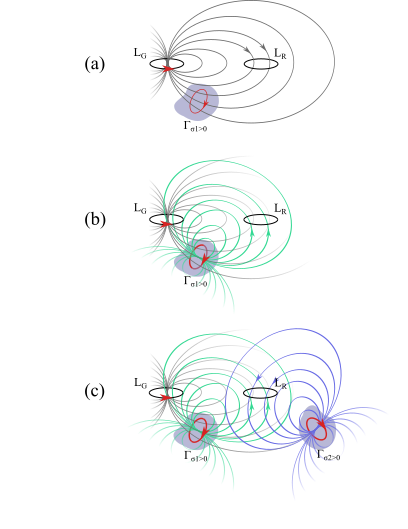
\includegraphics{./media/image2.png}
\caption{(a) The primary field \(B_{G}\) is created by driving
the generating coil \(L_{G}\) with an AC current. The receiving coil
\(L_{R}\) is penetrated by this field and a current is induced. A
conductive region \(\Gamma_{\sigma 1 > 0}\) is placed close to \(L_{G}\)
and \(L_{R}\).\(\ \Gamma_{\sigma 1 > 0}\) is penetrated by field lines
generated in \(L_{G}\), causing the induction of eddy currents in the
conductive domain. (b) Eddy currents induced in
\(\Gamma_{\sigma 1 > 0}\) create a secondary magnetic field \(\Delta\mathbf{B}\)
opposing the generating field. The magnetic fields \(\mathbf{B}_{G}\)
and \(\Delta\mathbf{B}\) superpose and can be measured using the
receiving coil \(L_{R}\). (c) A second conductive region
\(\Gamma_{\sigma 2 > 0}\) is placed close to \(L_{R}\). As in (b), this
conductive region is penetrated by field lines of \(B_{G}\) and eddy
currents form in \(\Gamma_{\sigma 2 > 0}\). Note how the directions of
secondary field lines at the receiver depend on the location of the
conductive region where they originate.}
\label{fig:coupling-model}
\end{figure}

\subsection{Field distributions in simple
geometry}\label{field-distributions-in-simple-geometry}

Simulated (CST Studio 2024, Frequency Domain Solver, simulation volume
\(300 \times 300 \times 300\ {mm}^{3}\))) field distributions for a
single generator and conductive region \(\Gamma_{\sigma > 0}\), like in
Figure~\ref{fig:coupling-model}b are shown in Figure~\ref{fig:simple-geometry-fields}: The conductive region is modeled as a
sphere of diameter \(d = 140mm\) having conductivity
\(\sigma = 0.733S/m\) (Heart material from CST Studio Database). The
circular generator coil (d=22mm) is excited with a broadband excitation
(0-150MHz). Figure~\ref{fig:simple-geometry-fields}a shows the magnetic (\(\mathbf{H}(x,y,z = const)\))
field distribution in absolute values. Note the rapid drop-off of both
fields with distance to the generator coil.

As noted above, the small size of the loop compared to the wavelength
results in a weak electric field. Integrating over the resulting
electric and magnetic energy density fields in this simulation showed,
that only 0.1\% of all energy deposited in the simulation region comes
from the electrical field.

To better visualize the perturbance of the magnetic field
\(\mathbf{B}_{g}\) due to the presence of the conductive region and the
eddy currents generated therein, we plot the difference
\(\Delta\mathbf{H =}\mathbf{H}_{object} - \mathbf{H}_{vacuum}\) in
Figure~\ref{fig:simple-geometry-fields}b, while Figure~\ref{fig:simple-geometry-fields}c shows the induced current density
\(\mathbf{J}(x,y,z = const)\).

For better visibility, \(\Delta\mathbf{H}\) is plotted in logarithmic
scale. Note how the induced currents, while only present within the
object boundaries, create a magnetic field extending through the whole
simulation volume. The resulting modulation of the magnetic field can be
sensed anywhere within the volume but is most pronounced close to the
object. Consequently, changes in the distribution of conductive tissues
and thus, signal modulation can be seen in the entire examination volume
and most, if not all receive coils will receive signal modulation.

In practice, this means that each coil will receive a motion signal that
is a mixture of respiratory, cardiac and other (in)voluntary motions
where every motion has a different amplitude and phase modulation
pattern over the receive channels. This difference forms the basis of
separating the motion types by channel combination in the processing of
the received signal \cite{Bacher2017CardiacStudy, Bacher2020PerformanceFramework}

\begin{figure}
\centering
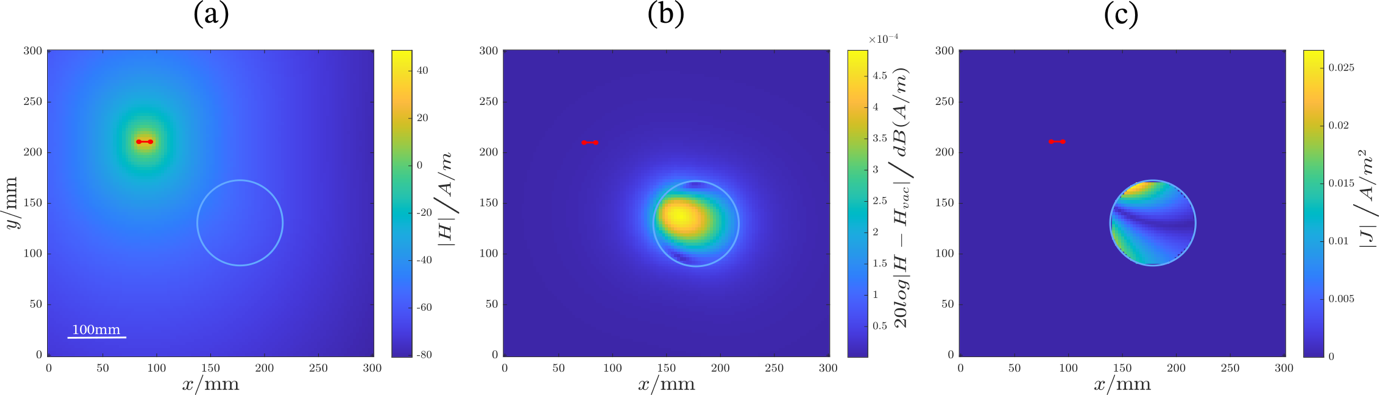
\includegraphics{./media/image3.png}
\caption{(a) Absolute magnetic field \(|\mathbf{H|}\), (b)
absolute magnetic difference
\(|\mathrm{\Delta}H| = |H| - {|H}_{vacuum}|\) to vacuum and (c) induced
absolute current density \(|\mathbf{J}|\) field distributions with a
spherical conductive object (blue outline) present. Magnetic difference
field is displayed in logarithmic scale for better visibility. The red
``barbell'' marks the position of the generating coil \(L_{G}\),
d=22mm.}
\label{fig:simple-geometry-fields}
\end{figure}

\section{Methods}\label{methods-1}

\subsection{Simulations \& Experiments}\label{simulations-experiments}

The resulting in-vivo signal in each receive-coil is a superposition of
primarily respiratory and cardiac motion but is also sensitive to other
motion, such as movement of limbs and presumably also peristaltic
motion. In practice, we obtain stable respiratory and cardiac signals by
linear combination of receiving coils using blind source separation
methods such as ICA (independent component analysis) \cite{Bacher2020PerformanceFramework, BacherRetrospectiveCohort}. To
better understand and demonstrate the underlying physical processes,
that is, the interplay of changes in conductivity and permittivity due
to tissue displacement through motion in the receiving coils field of
view, we used numerical electromagnetic simulations using the Finite
Integration Technique (FIT) which discretizes Maxwell's equations in
both space and time to solve electromagnetic problems.

Simulations were performed on a realistic human torso model to
demonstrate the physical processes that result in the received motion
modulated signal and how this signal relates to cardiac motion.

\subsection{Digital human phantom}\label{digital-human-phantom}

We simulated a realistic human torso (XCat v2 phantom \cite{Segars20104DResearch}),
comprised of 30 different tissue types with their respective values for
conductivity and relative permittivity at frequencies from 10 to 150MHz
to include the three most common field strengths of 0.55T, 1.5T and 3T.

The XCat phantom can simulate realistic anatomical deformations due to
breathing, heartbeat or both. We simulated geometric changes over a
complete cardiac cycle at 12 distinct, equally spaced timepoints. Tissue
properties were taken from CST Studios built-in database where
available. Tissue parameters not available in the CST library were taken
from the IT'IS database \cite{HasgallITIS2018}. and frequency dependence was modeled
using CST Studios Dielectric Dispersion Fit.

\revorange{Table~\ref{tab:tissue-properties} lists the tissue electromagnetic properties used in the simulations. Values are based on the parametric models of Gabriel et al.\ \cite{Gabriel1996Dielectric} as compiled by Andreuccetti et al.\ \cite{Andreuccetti1997}, evaluated at 100\,MHz. CST Studio's Dielectric Dispersion Fit was applied to adjust all properties to the exact simulation frequencies (62.5\,MHz for 1.5T and 122.5\,MHz for 3T). All tissues are modeled with isotropic, scalar conductivity and permittivity. Pericardium properties were taken from the NICT tissue database \cite{NICT2023Tissues}.}

\begin{table}[htbp]
\centering
\revorange{\caption{Electromagnetic tissue properties at 100\,MHz used in the simulation.}\label{tab:tissue-properties}}
\revorange{
\begin{tabular}{l r r}
\hline
\textbf{Tissue} & $\varepsilon_r$ & $\sigma$ (S/m) \\
\hline
Blood             & 76.82 & 1.233 \\
Heart muscle      & 90.82 & 0.733 \\
Pericardium       & 29.50 & 0.246 \\
Lung (avg.)       & 49.38 & 0.434 \\
Liver             & 69.02 & 0.487 \\
Muscle            & 65.97 & 0.708 \\
Fat               &  6.07 & 0.036 \\
Skin (avg.)       & 69.45 & 0.507 \\
Pancreas          & 68.81 & 0.794 \\
Stomach wall      & 77.90 & 0.900 \\
Small intestine   & 96.55 & 1.655 \\
Large intestine   & 96.55 & 1.655 \\
Gall bladder      & 94.96 & 1.541 \\
Kidney            & 98.09 & 0.811 \\
Spleen            & 90.66 & 0.802 \\
Spinal cord       & 47.27 & 0.338 \\
Bone cortical     & 15.28 & 0.064 \\
Bone spongiosa    & 27.63 & 0.173 \\
Bone medullary    & 27.63 & 0.173 \\
Air (inside body) &  1.00 & 0.000 \\
\hline
\end{tabular}
}
\end{table}

The PT generator coil was placed anterior to the beating in-silico
heart. A total of 28 rectangular receive coils were modeled to simulate
an anterior and posterior surface coil array, like those used in a
typical CMRI exam. We used CST Studios Time Domain Solver with the
following settings:

\begin{itemize}
\item
  Mesh type: Hexahedral
\item
  Simulation Volume: \(550\  \times 550\  \times 677\ mm^{3}\)
\item
  Accuracy: -80dB
\item
  Mesh refinement: Expert system based with mesh increment of 5,
  resulting in a High Frequency Type mesh with 223.5 million meshcells
\item
  Boundary Conditions: magnetic (Ht=0)
\item
  S-parameter ports with impedance 50 Ohm for Tx and Rx elements, input
  power 1W
\item
  Frequency range: 10MHz-150MHz, step size 0.14MHz
\item
  Field probes for magnetic (H), electric (E) and current density (J)
  fields at 62.5 and 122.5MHz
\end{itemize}

The geometric setup of the phantom, PT generator loop and Rx elements is
shown in Figure~\ref{fig:phantom-setup}.

The transmit loop was modeled as a circular PEC (perfect electric
conductor) element with d=30mm. Receive loops were modeled as
rectangular PEC elements arranged in posterior and anterior arrays
without overlap.

The generator is integrated in the anterior coil and is positioned on
top of the heart, consistent with the in-vivo placement. For geometric
decoupling it is placed in between the two central coil elements 7 \rev{and} 8.

Twelve Rx coils were placed anterior and 16 posterior of the phantom,
simulating elements of a typical surface coil array used in abdominal or
cardiac MRI.

Simulation was performed on a distributed computing cluster with 2x22
cores @ 2.2GHz, 512GB of memory and using NVIDIA GPUs (Quadro GV100,
NVIDIA Corporation, Santa Clara, CA, driver version 441.12). Simulation
took approximately 6h per frame.

The simulated (\(\mathbf{H}(x,y,z)\) and \(\mathbf{E}(x,y,z)\)) and
\(\mathbf{J}(x,y,z)\)) fields and calculated S-parameter curves in the
frequency range 10MHz -- 150MHz were then exported to Matlab 2023a
(MathWorks, Natick, MA) for analysis.

\begin{figure}
\centering
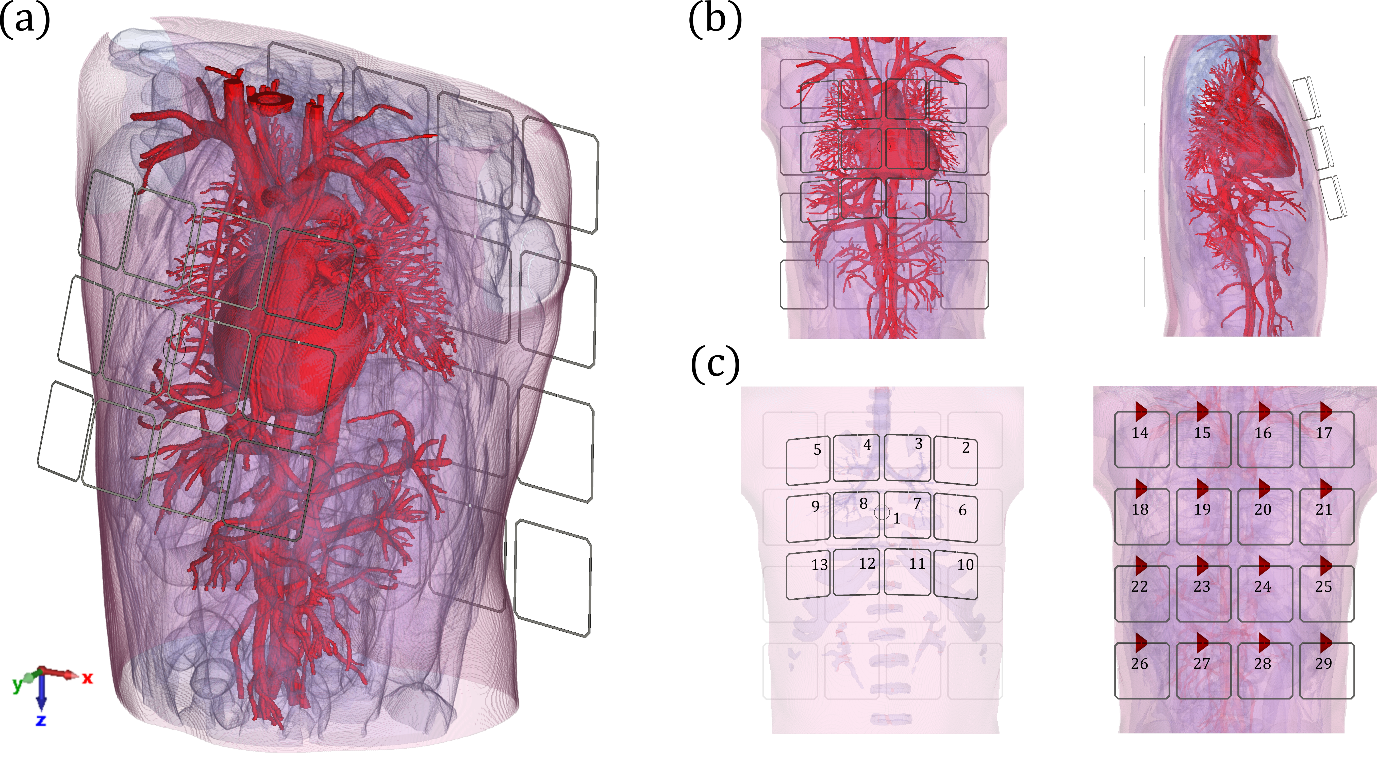
\includegraphics{./media/image4.png}
\caption{Geometric setup of the virtual human phantom. (a) 3D
view and (b) frontal and side view of the virtual human phantom and the
receive coils. (c) Position and port numbers of PT generator coil (1),
anterior Rx elements (2-13) and posterior Rx elements (14-29).}
\label{fig:phantom-setup}
\end{figure}

To visualize the field variations causing this received signal, we
created transverse and sagittal planes through the heart from the
simulated H-field. To further visualize how conductive tissues affect
the field distribution, we further subtracted the generating field,
obtained from one simulation run where all tissues were set to the
background air material. Additionally, the current density (J) field in
these two slices was extracted from the simulated J-field.

\revgreen{To visualize the temporal evolution of the secondary magnetic field due to cardiac motion, we computed the difference $\Delta\mathbf{H}(t) = \mathbf{H}(t) - \mathbf{H}(t_1) - \mathbf{B}_G$ at each timepoint relative to the first frame (start of systole) in a transverse plane through the heart, with the static generator field $B_G$ subtracted.}

S-parameter calculation was performed for each timeframe of the virtual
phantoms cardiac cycle. \rev{Scattering parameters (S-parameters) characterize the transmission and reflection of electromagnetic waves in a multi-port network. In our setup, $S_{n,1}$ represents the complex transmission coefficient from the PT source (port 1) to receive coil element $n$ i.e., the ratio of the wave amplitude received at port $n$ to the wave amplitude incident at port 1, with all other ports terminated in their characteristic impedance $Z_0 = 50\,\Omega$. Changes in the tissue distribution between the transmit and receive ports alter $S_{n,1}$; the relative change $\Delta S_{n,1}/S_{n,1}$ between cardiac phases directly quantifies the modulation depth (see Appendix, Eq.~\ref{SParamCouplingSimplified}).}

To evaluate the change in received signal in
each Rx coil due to cardiac motion, we evaluated the S-parameter at
typical frequencies (122.5MHz for 3T systems and 62.5MHz for 1.5T
systems) in time direction and compared to the known volume curve of the
virtual phantom.

To investigate the influence of operating frequency on signal
modulation, S-parameter curves were analyzed over the whole frequency
range (10-150MHz) with regard to modulation depth, defined as the change
in received signal amplitude \(s_{PT}\) from full expansion (frame 1) to
maximum contraction (frame 7) as a percentage of the mean received
amplitude over the whole cardiac cycle:

\begin{equation}
\label{eq:mod-depth-mag}
m_{d,\mathrm{mag}} = \frac{s_{PT}(t = 1) - s_{PT}(t = 7)}{\mathrm{mean}\!\left(s_{PT}(t)\right)} \cdot 100\%
\end{equation}

Modulation of signal phase was analyzed by defining phase modulation
depth as the difference between the phase in frame 1 and frame 7:

\begin{equation}
\label{eq:mod-depth-phase}
m_{D,\mathrm{phase}} = \angle s_{PT}(t = 1) - \angle s_{PT}(t = 7)
\end{equation}

Note that, as discussed previously, the modulation can be either
positive (decrease in received signal as cardiac volume decreases) or
positive.

\revgreen{To quantify the relationship between signal modulation and cardiac motion, we computed the Pearson correlation coefficient $R$ between each channel's S-parameter curve (magnitude and phase, respectively) and the total heart volume ground truth. The heart volume was extracted from the voxel model by summing all voxels belonging to cardiac tissue types (heart muscle, blood, pericardium) across all 12 cardiac phases. A positive $R$ indicates that the signal quantity increases with cardiac volume; a negative $R$ indicates an inverse relationship. We report $|R|$ (mean $\pm$ SD) across channel groups and per-channel signed $R$ values.}

\subsection{Experimental validation}
%\label{experimental-validation}

\revbrown{
To validate the simulation predictions experimentally, S-parameter measurements were performed on three healthy volunteers (\mbox{Table~\ref{tab:volunteers}}) using an experimental system comprising PT generation hardware, a multi-channel digital receiver, and an interface for clinical product coil arrays. The system was installed in a shielded enclosure with conductive walls of dimensions comparable to a clinical MRI bore, preserving the waveguide boundary conditions discussed in Section~\ref{theory}. No static magnetic field was present.}

\begin{table}[htbp]
\centering
\caption{Volunteer characteristics.}
\label{tab:volunteers}
\begin{tabular}{lccccc}
\hline
Volunteer & Gender & Age & Height (cm) & Weight (kg) & Coil configuration \\
\hline
V1 & [M/F] & [AGE] & [HEIGHT] & [WEIGHT] & Body~18 + Spine~24 \\
V2 & [M/F] & [AGE] & [HEIGHT] & [WEIGHT] & Body~12 + Spine~24 \\
V3 & [M/F] & [AGE] & [HEIGHT] & [WEIGHT] & Body~18 + Spine~24 \\
\hline
\end{tabular}
\end{table}

\revbrown{
The PT generator, a small loop antenna integrated into the anterior coil array housing, was driven at 0\,dBm (1\,mW) at a carrier frequency of 62.5\,MHz (corresponding to 1.5\,T). Receive coil arrays consisted of either a Biomatrix Body~18 or Body~12 (anterior) combined with a Spine~24 array (posterior), yielding 18+9 or 12+12 active receive channels respectively.}

\revbrown{
The receiver was characterised by mapping digital output values to analog input power: signals ranging from $-120$\,dBm (noise floor) to $-35$\,dBm (onset of receiver nonlinearity) were directly fed into each coil element's low-noise preamplifier input, establishing a calibrated 85\,dB linear dynamic range. Scattering parameters $S_{1,n}$\,(dB) were then computed from the known transmit power (0\,dBm) and the calibrated received signal level in each channel.}

\revbrown{
Volunteers were positioned supine and instructed to hold their breath. Raw per-channel PT magnitude and phase signals, sampled at 2\,kHz, were recorded continuously. Within each breathhold segment, mild baseline drifts were removed by polynomial detrending (preserving mean amplitudes). Cardiac cycles were segmented using peak detection on a reference channel with strong cardiac modulation, and individual cycles were aligned and averaged to produce mean cardiac waveforms per channel. Confidence intervals (95\,\% CI) were computed as $\bar{x} \pm 1.96\,\sigma_\mathrm{noise}$, where $\sigma_\mathrm{noise}$ is the standard deviation of the residual after cycle averaging, providing a direct measure of the per-channel noise floor relative to the cardiac modulation amplitude.}

\revbrown{
Modulation depth was defined analogously to the simulation (Eq.~\ref{eq:mod-depth-mag}): the peak-to-peak excursion of the averaged cardiac waveform as a percentage of the mean signal level, evaluated in both raw amplitude, dBm, and $S_{1,n}$\,(dB) domains.}

% [FIGURE PLACEHOLDER: Experimental setup photograph or schematic diagram]
% \begin{figure}[htbp]
% \centering
% \includegraphics[width=\columnwidth]{./media/exp_setup.png}
% \caption{Experimental setup for S-parameter validation measurements.}
% \label{fig:exp-setup}
% \end{figure}


\section{\texorpdfstring{Results }{Results }}\label{results-1}

\subsection{Electric and magnetic
field}\label{electric-and-magnetic-field}

Figure~\ref{fig:field-slices} shows quantitative maps for absolute (a) magnetic field
strength difference to the unloaded case (air)
\(|\mathrm{\Delta}H| = |H - H_{air}|\) and (b) absolute current density
\(|J|\) in coronal (top) and \rev{sagittal} (bottom) slices through the
virtual phantoms heart. The outline of the heart is shown by a white
curve, the position of the PT generator loop is indicated by a red
circle or barbell.

Note how the induced current density is strongest close to the PT
generator (red), which is positioned some millimeters anterior to the
heart. The change in magnetic field strength is strongest in the
vicinity of the heart. Note that the generative field falls off with
distance cubed from the generator loop (Biot-Savart law) and
consequently so does the secondary field \(\Delta\mathbf{B}\) and the
induced current density \(\mathbf{J}\).

\revgreen{The resulting animated difference maps of the secondary magnetic field over the cardiac cycle are shown in Supplementary Figure 1.}

\begin{figure}
\centering
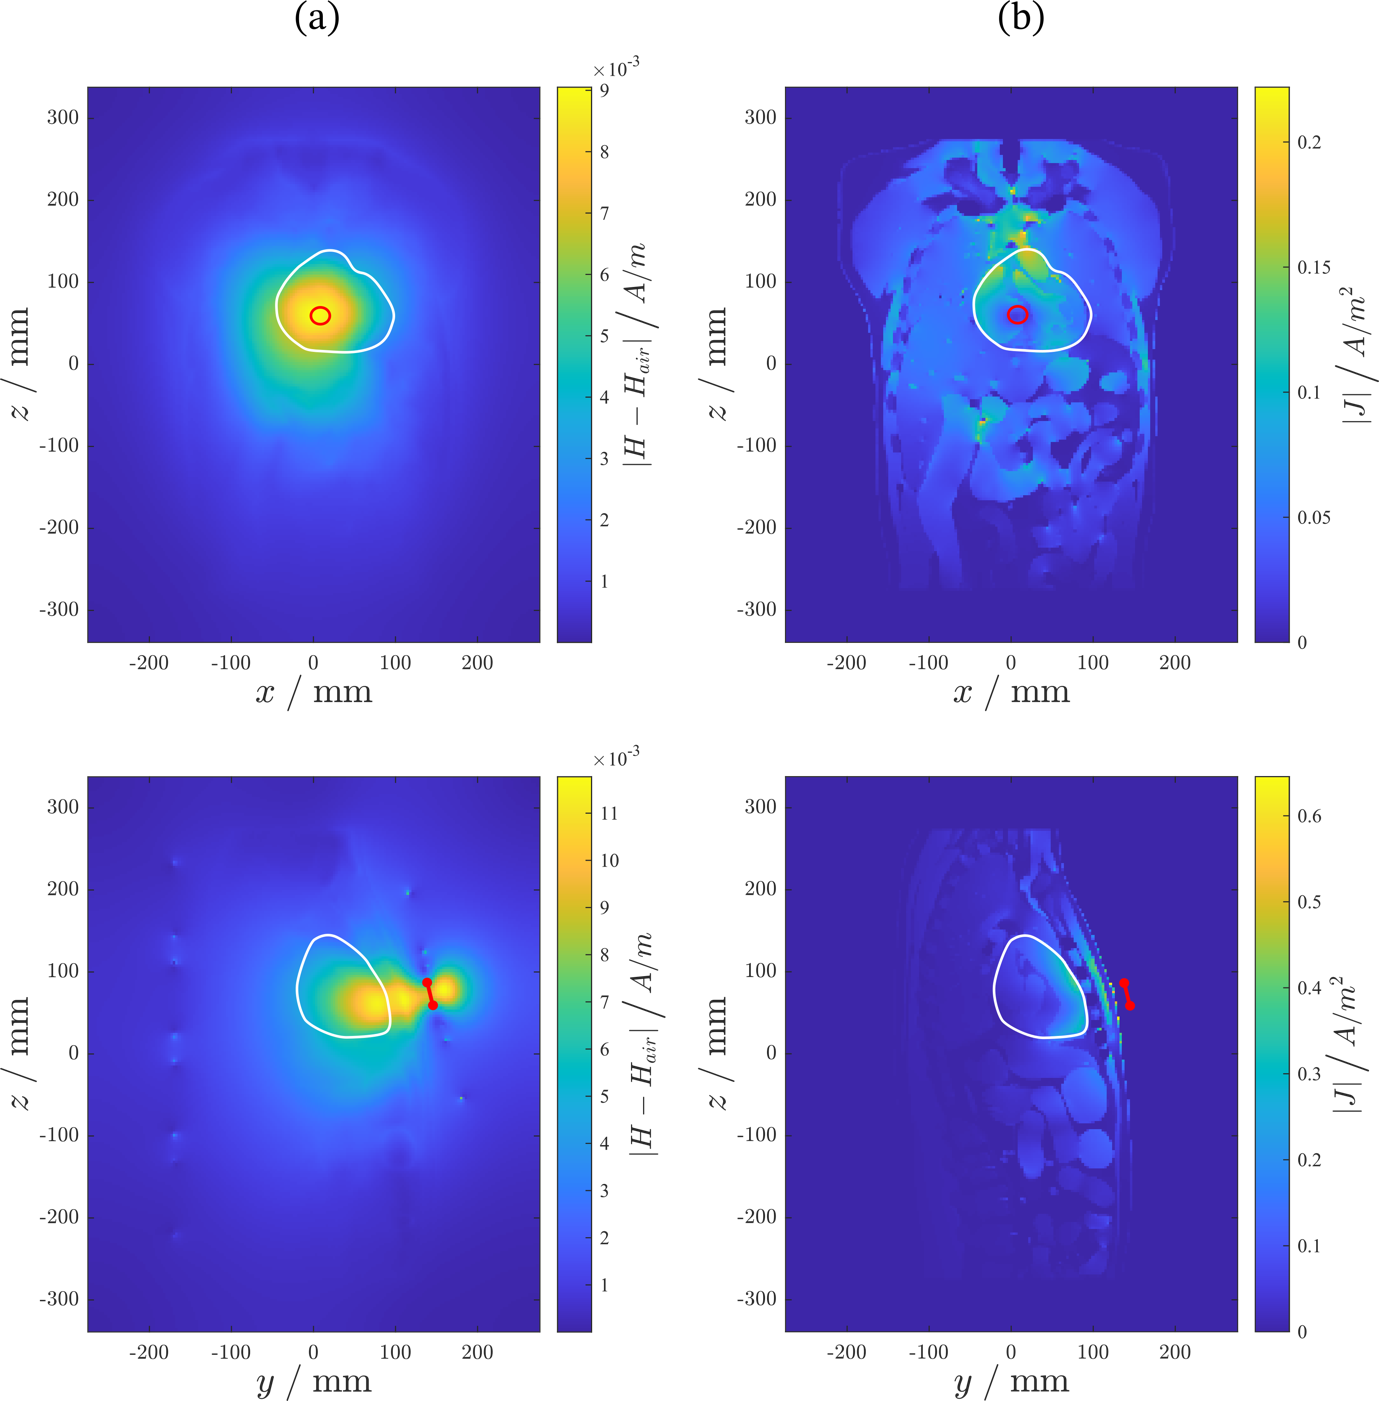
\includegraphics{./media/image5.png}
\caption{Coronal (top) and sagittal (bottom) slices through
the heart of the virtual human phantom. (a) Absolute induced current
density $\lVert\mathbf{J}\rVert$ in A/m$^{2}$ and (b) absolute secondary magnetic field $\lVert\Delta\mathbf{H}\rVert$
in A/m. The red circle and barbell denote the position of the PT
generator loop; the white curve shows the outline of the heart for
reference.}
\label{fig:field-slices}
\end{figure}

\subsection{Signal modulation \& relation to cardiac
motion}\label{signal-modulation-relation-to-cardiac-motion}

The received signal over time is plotted, for all individual Rx
elements, in Figures~\ref{fig:rx-magnitude-62} and~\ref{fig:rx-magnitude-122} as complex magnitude in dBm (rescaled to
1mW input power) and in Figures~\ref{fig:rx-phase-62} and~\ref{fig:rx-phase-122} as phase modulation. \revgreen{Magnitude and phase modulation depths are defined in Eqs.~\eqref{eq:mod-depth-mag} and~\eqref{eq:mod-depth-phase}, respectively.}

Modulation depths of individual channels are compared graphically in
Figure~\ref{fig:mod-depth-bars-mag} for magnitude and in Figure~\ref{fig:mod-depth-bars-phase} for phase and summarized in
Figure~\ref{fig:mod-depth-summary}\revred{, with per-channel correlation coefficients listed in Table~\ref{tab:per-channel}}.

\revgreen{Results are presented at 62.5\,MHz and 122.5\,MHz, corresponding to PT frequencies close to Larmor frequencies but outside the imaging bandwidth at 1.5\,T and 3\,T, respectively.}

\revgreen{Correlation results between S-parameter modulation and heart volume are summarized in Table~\ref{tab:correlation}.}

\begin{table}[ht]
\centering
\revred{
\caption{Pearson correlation coefficient $|R|$ and modulation depth $m_D$ between simulated S-parameter curves and heart volume ground truth, given as mean $\pm$ SD across channels. Magnitude modulation depth is in percent; phase modulation depth in radians.}
\label{tab:correlation}
\begin{tabular}{ll|cc|cc}
\hline
 & & \multicolumn{2}{c|}{\textbf{62.5 MHz (1.5T)}} & \multicolumn{2}{c}{\textbf{122.5 MHz (3T)}} \\
\textbf{Array} & \textbf{Signal} & $|R|$ & $m_D$ & $|R|$ & $m_D$ \\
\hline
Anterior (S2--S13) & Mag. [\%] & $0.94 \pm 0.20$ & $0.79 \pm 0.68$ & $0.94 \pm 0.18$ & $2.00 \pm 2.14$ \\
                   & Phase [rad] & $0.90 \pm 0.28$ & $0.004 \pm 0.004$ & $0.98 \pm 0.05$ & $0.017 \pm 0.023$ \\
Posterior (S14--S29) & Mag. [\%] & $0.99 \pm 0.03$ & $0.85 \pm 0.79$ & $0.97 \pm 0.06$ & $1.80 \pm 2.23$ \\
                     & Phase [rad] & $0.99 \pm 0.03$ & $0.005 \pm 0.005$ & $0.99 \pm 0.02$ & $0.035 \pm 0.041$ \\
\hline
All channels & Mag. [\%] & $0.97 \pm 0.13$ & $0.83 \pm 0.73$ & $0.96 \pm 0.13$ & $1.89 \pm 2.15$ \\
             & Phase [rad] & $0.95 \pm 0.18$ & $0.004 \pm 0.005$ & $0.98 \pm 0.04$ & $0.027 \pm 0.035$ \\
\hline
\end{tabular}
}
\end{table}

\subsubsection{Magnitude modulation:}\label{magnitude-modulation}

Figures~\ref{fig:rx-magnitude-62} and~\ref{fig:rx-magnitude-122} show the received magnitude signal over time in dBm
(rescaled to 1mW input power) during one cardiac cycle, evaluated at
62.5 and 122.5MHz. \revred{Received signal curves show strong quantitative correlation to total cardiac volume ($|R| = 0.97 \pm 0.13$ at 62.5\,MHz, $|R| = 0.96 \pm 0.13$ at 122.5\,MHz, see Table~\ref{tab:correlation})}\revdel{Received signal curves correlate qualitatively
extremely well to total cardiac volume}, plotted in red, in all but one
anterior element.

Modulation depths (see also Figure~\ref{fig:mod-depth-summary} and Figures~\ref{fig:mod-depth-bars-mag} and~\ref{fig:mod-depth-bars-phase}) were found to be
slightly higher in the anterior elements at 122.5MHz (mean modulation
depth 0.14\% anterior vs. 0.12\% posterior) and almost similar at
62.5MHz (0.06\% anterior vs. 0.065\% posterior)\revred{. Per-channel modulation depths and signed correlation coefficients are listed in Table~\ref{tab:per-channel}.}

Direct coupling, i.e. mean received amplitudes as well as modulation
depths overall appear to increase roughly linearly with frequency --
doubling the frequency from 62.5 to 122.5MHz roughly doubled mean
modulation depth.

\subsubsection{Phase modulation:}\label{phase-modulation}

Figures~\ref{fig:rx-phase-62} and~\ref{fig:rx-phase-122} show the received phase signal over time at 62.5MHz and
122.5MHz in anterior and posterior elements. Phase modulation
(individual elements summarized in Figure~\ref{fig:mod-depth-summary} and Figures~\ref{fig:mod-depth-bars-mag} and~\ref{fig:mod-depth-bars-phase}) also
correlates very well quantitatively to cardiac volume ground truth.
Contrary to magnitude modulation depth, phase modulation depth increased
by a factor of 5 in anterior elements and 7 in posterior elements when
doubling the PT frequency.

\begin{figure}
\centering
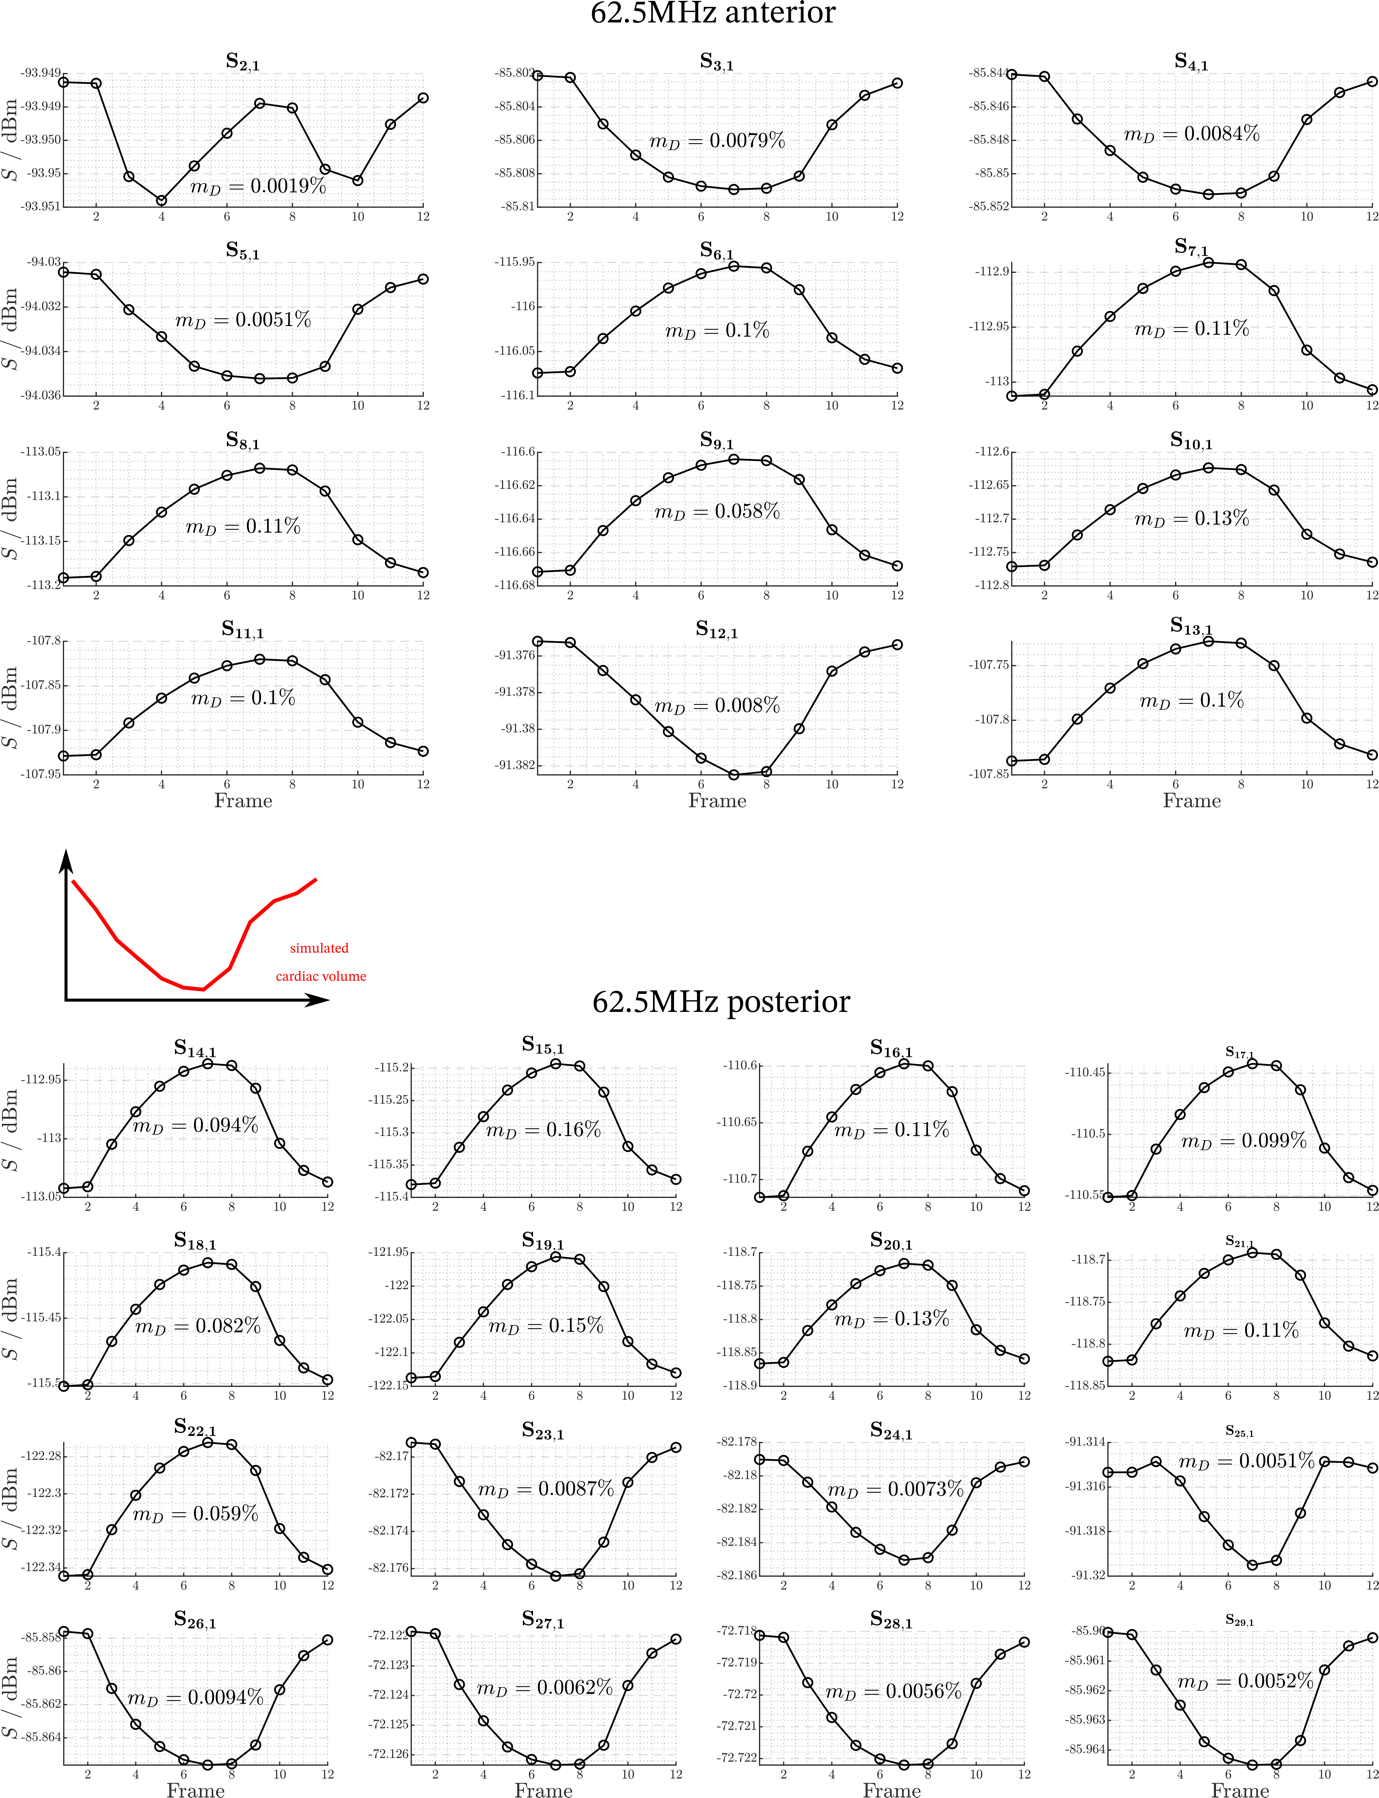
\includegraphics{./media/image6.png}
\caption{Received signal magnitude in dBm in anterior (top)
and posterior (bottom) Rx channels over time during one cardiac phase at
62.5MHz. Cardiac volume ground truth is shown in red.}
\label{fig:rx-magnitude-62}
\end{figure}

\begin{figure}
\centering
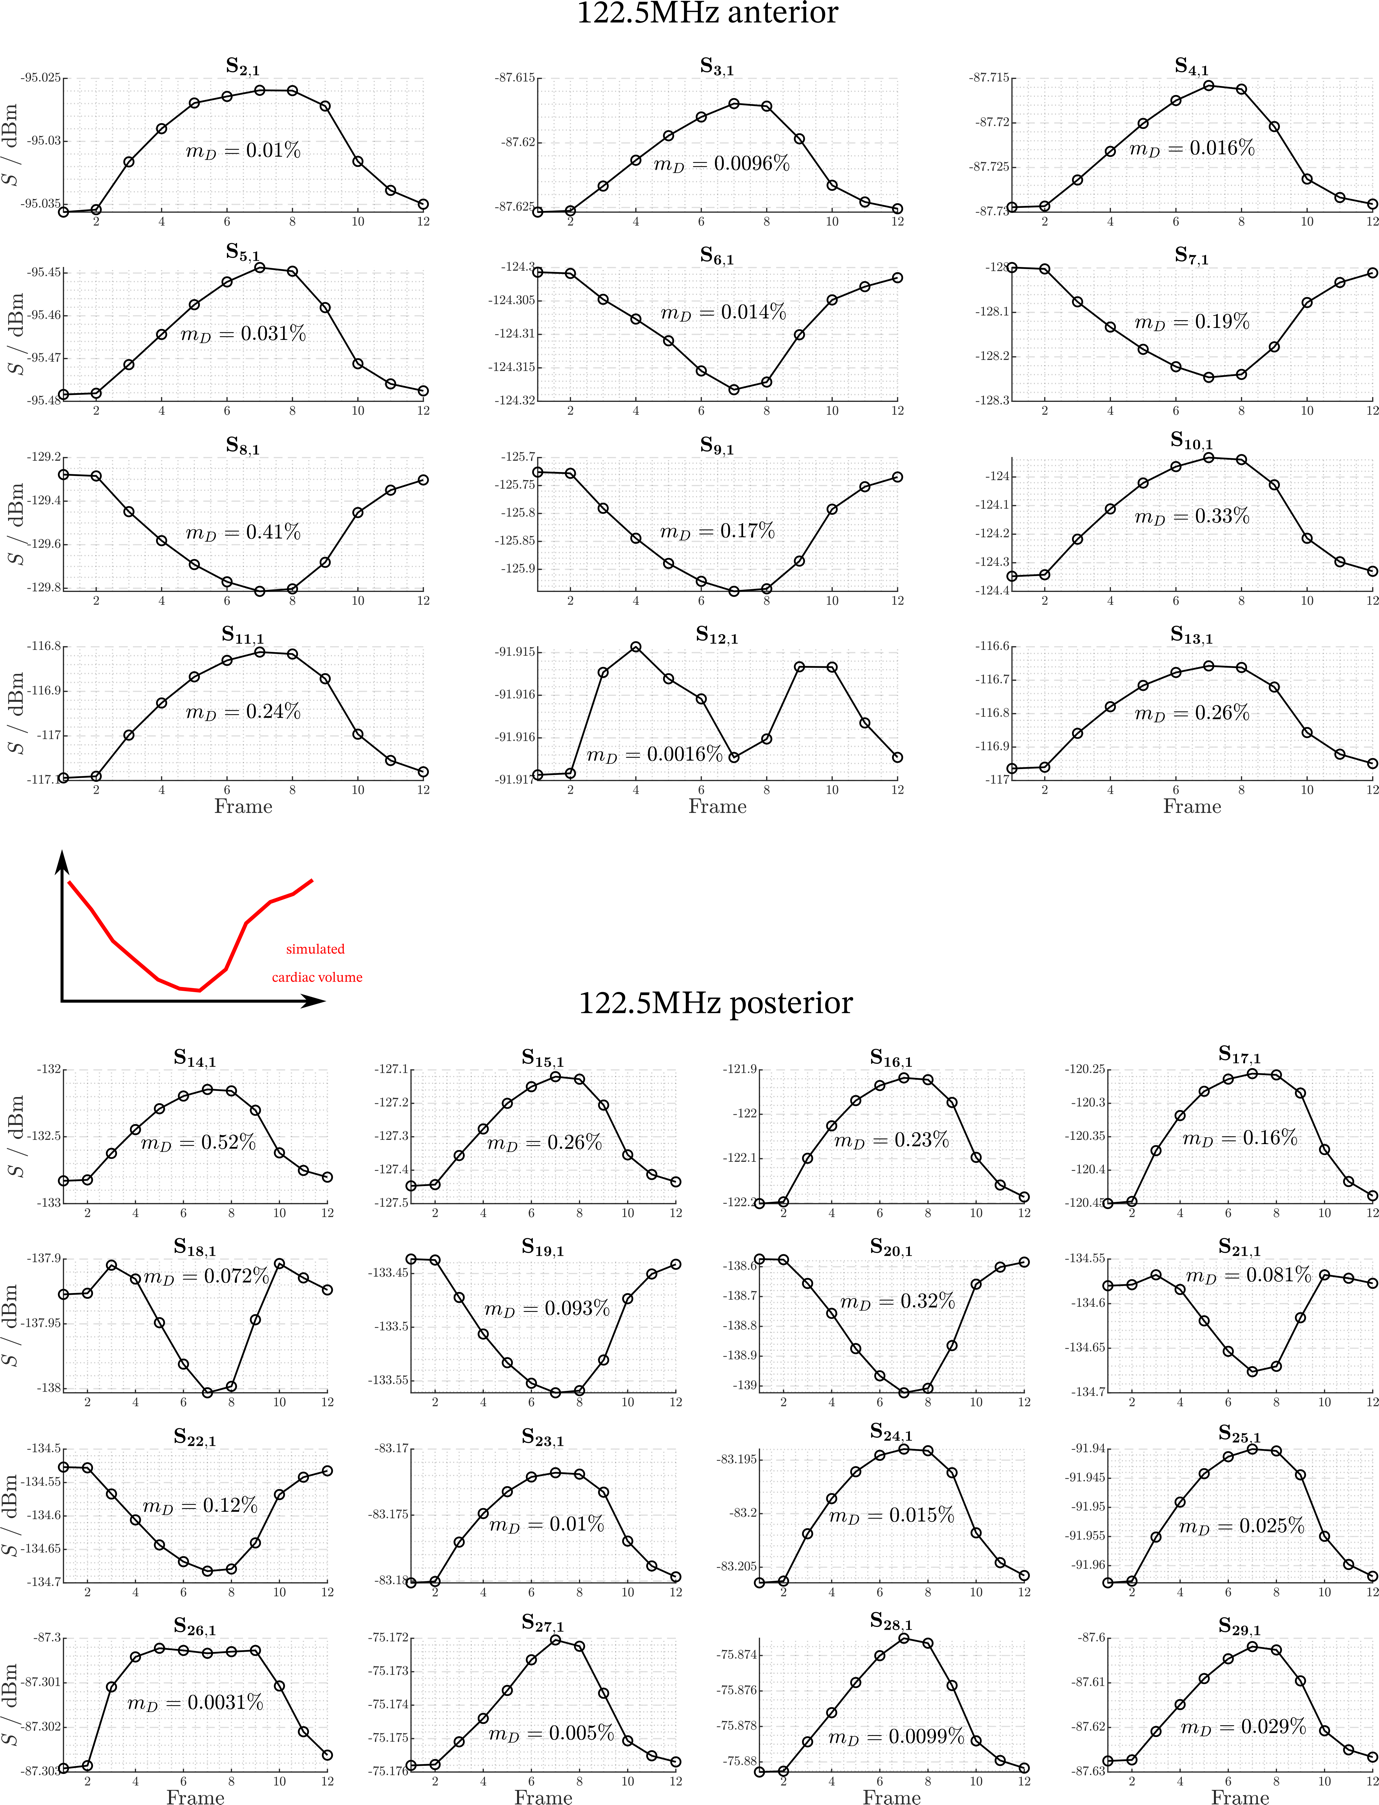
\includegraphics{./media/image7.png}
\caption{Received signal magnitude in dBm in anterior (top)
and posterior (bottom) Rx channels over time during one cardiac phase at
122.5MHz. Cardiac volume ground truth is shown in red.}
\label{fig:rx-magnitude-122}
\end{figure}

\begin{figure}
\centering
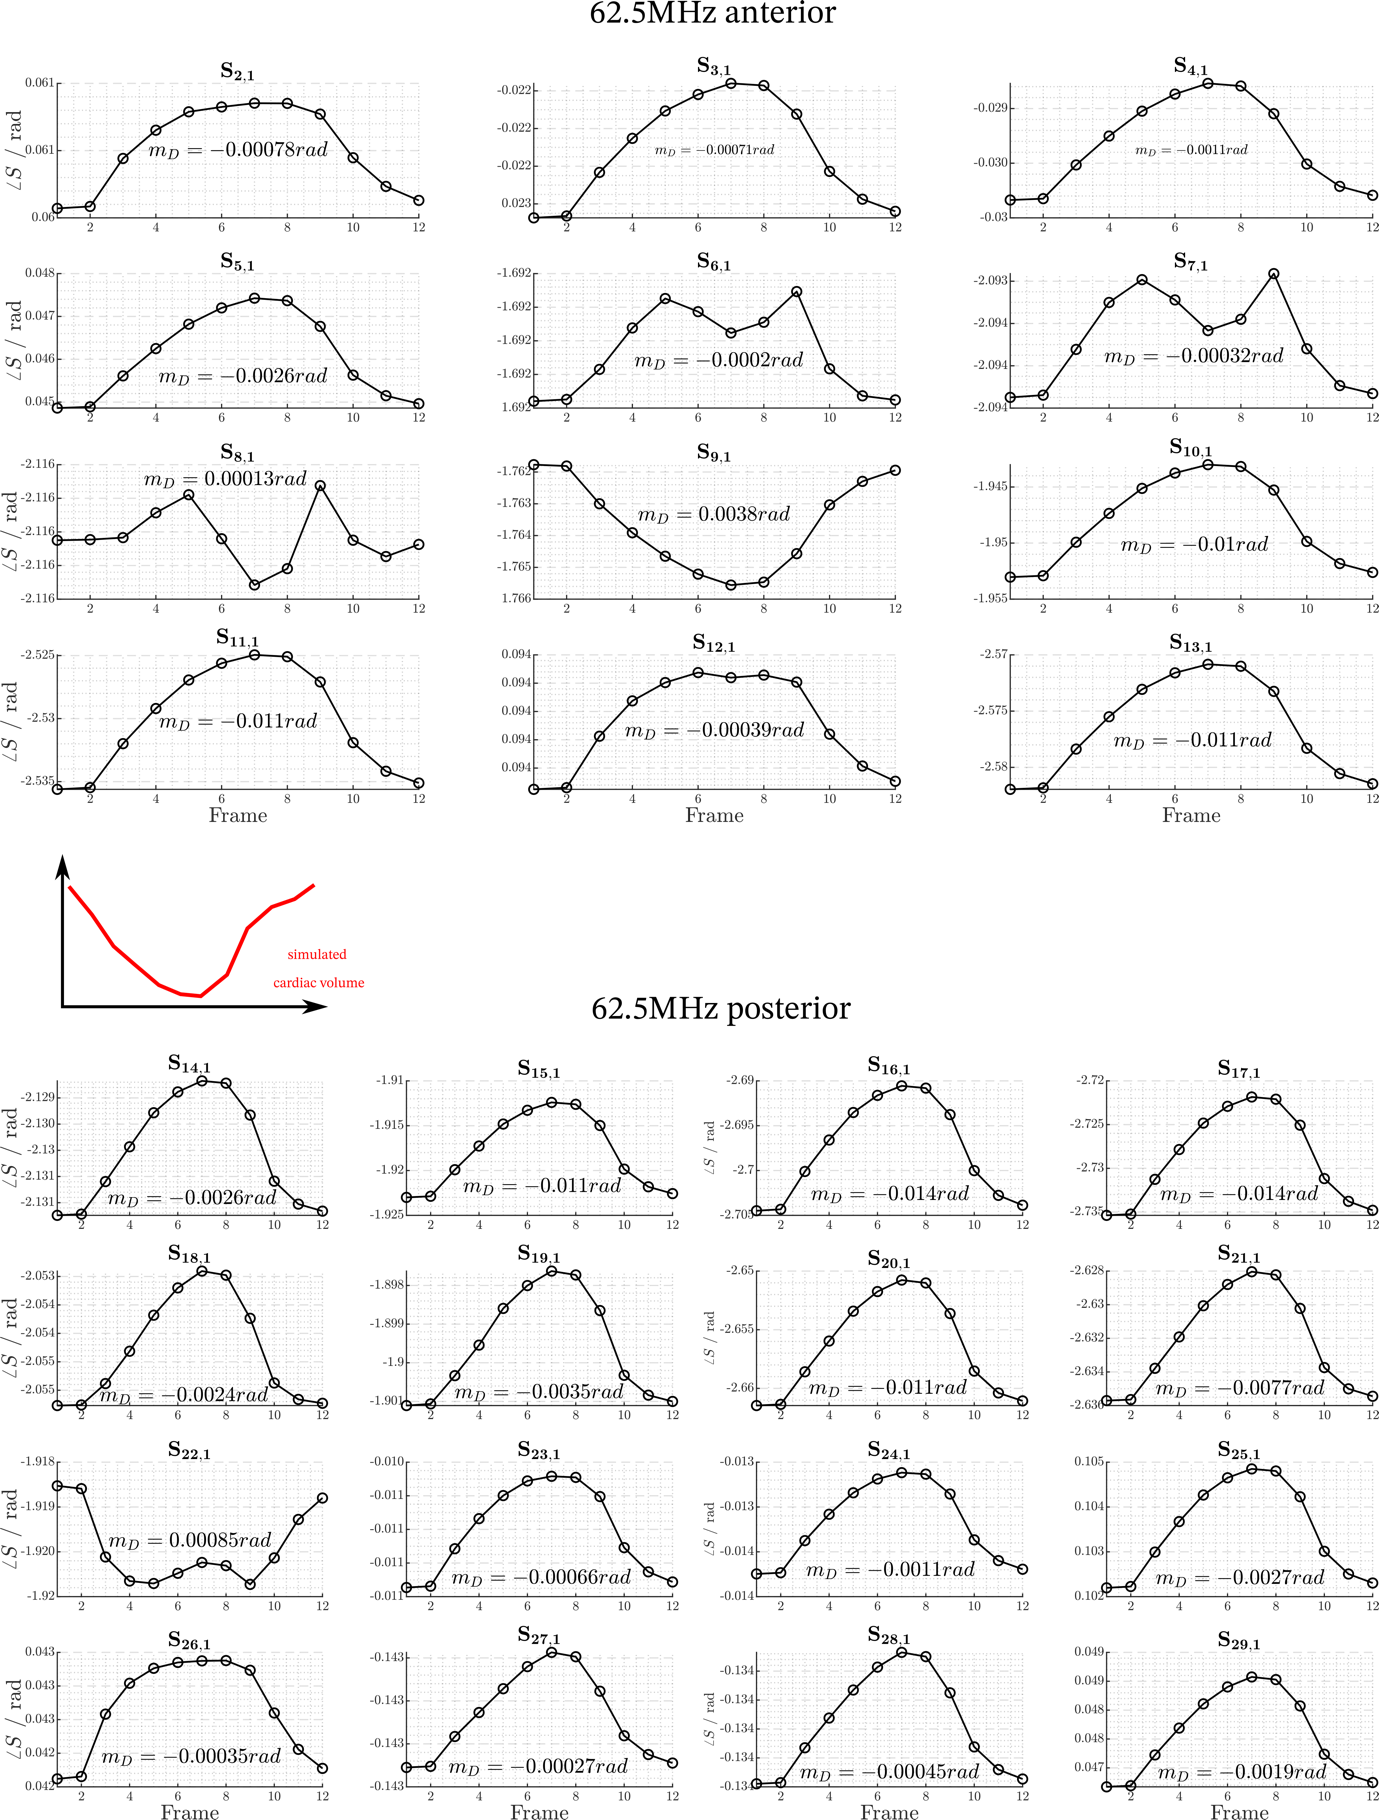
\includegraphics{./media/image8.png}
\caption{Received signal phase in radians in anterior (top)
and posterior (bottom) Rx channels over time during one cardiac phase at
62.5MHz. Cardiac volume ground truth is shown in red.}
\label{fig:rx-phase-62}
\end{figure}

\begin{figure}
\centering
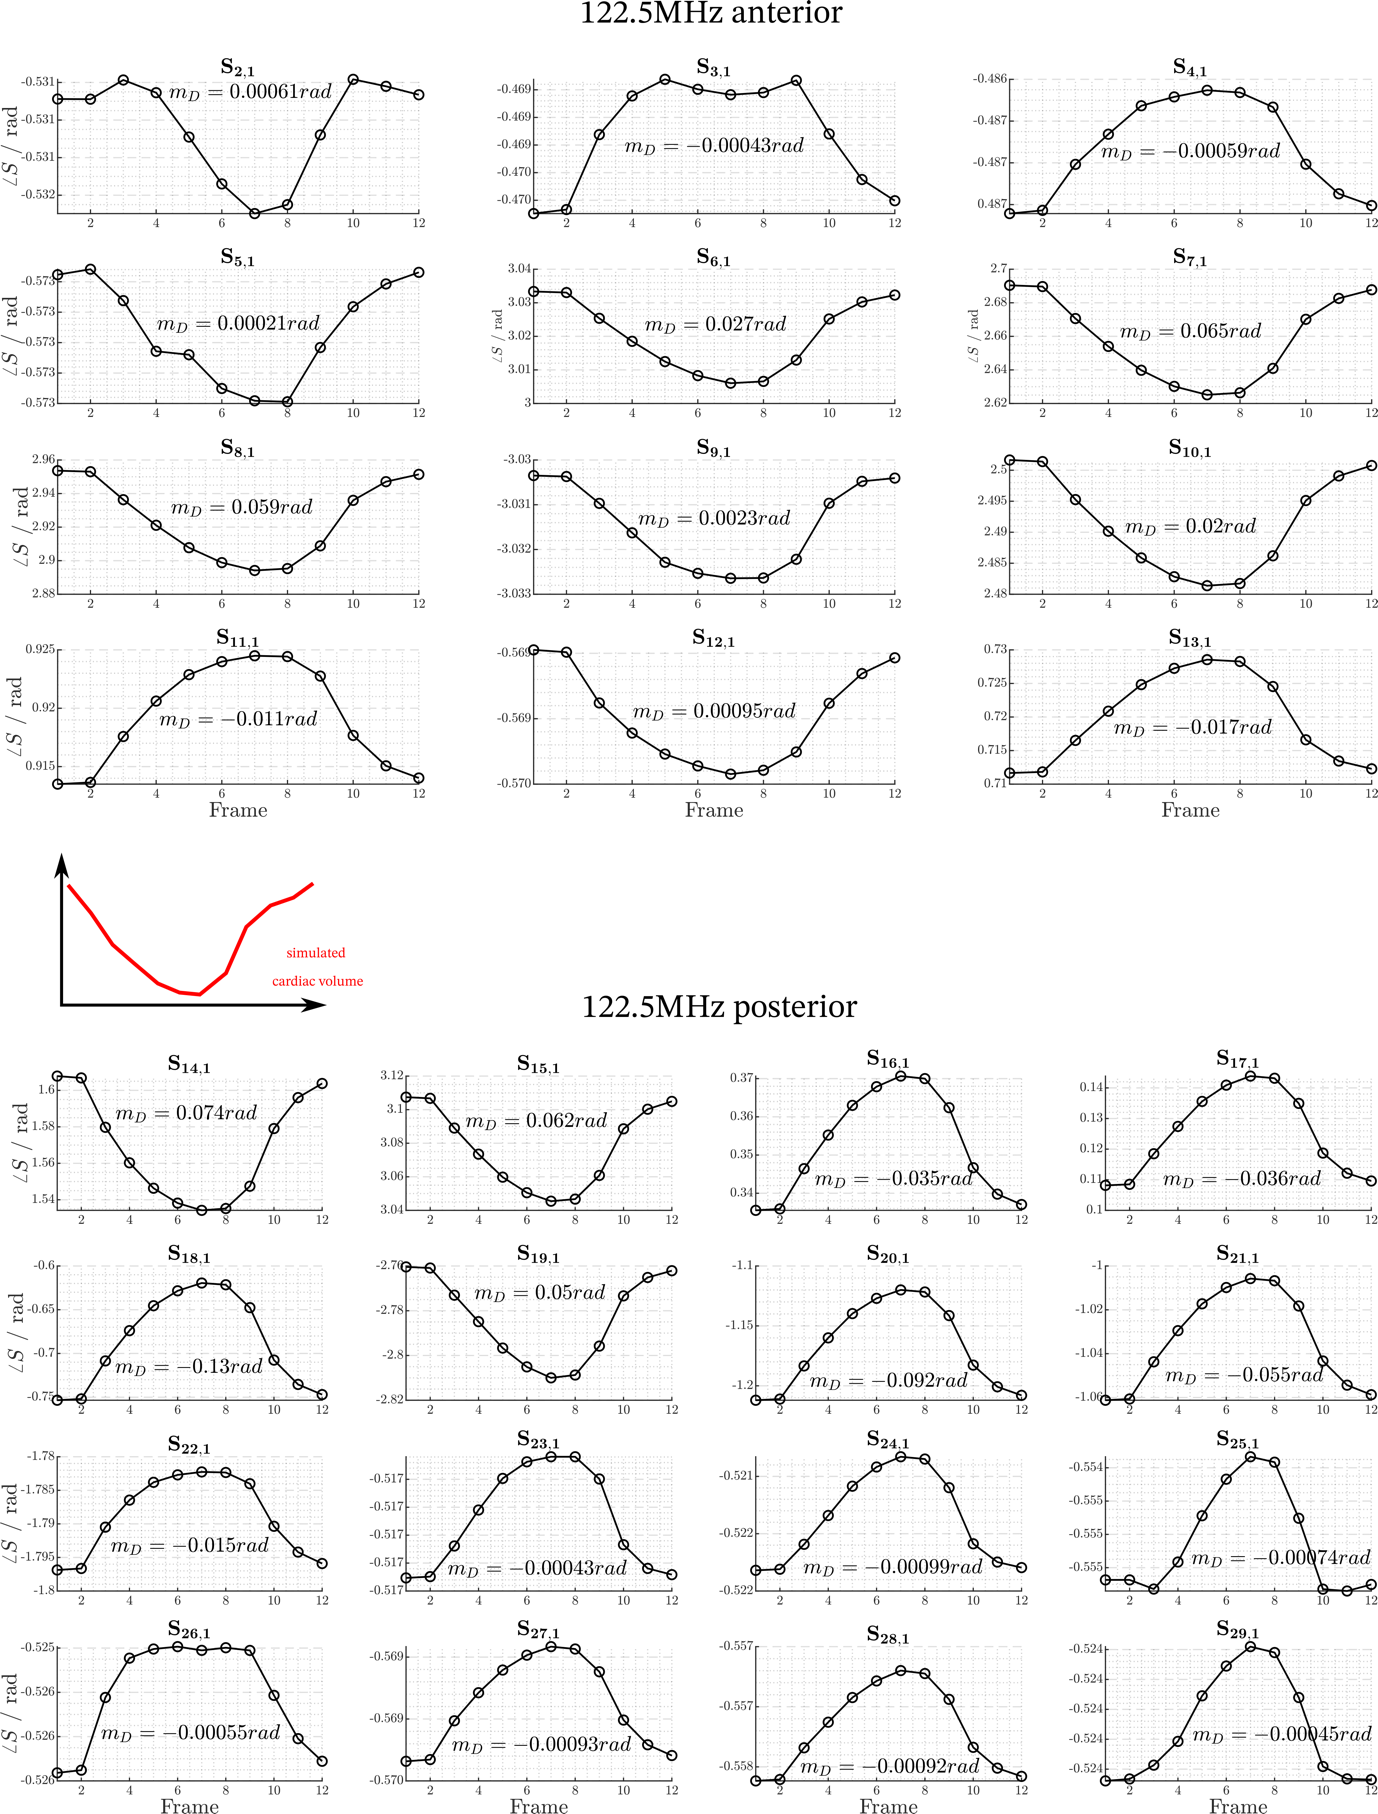
\includegraphics{./media/image9.png}
\caption{Received signal phase in radians in anterior (top)
and posterior (bottom) Rx channels over time during one cardiac phase at
62.5MHz. Cardiac volume ground truth is shown in red.}
\label{fig:rx-phase-122}
\end{figure}

\begin{figure}
\centering
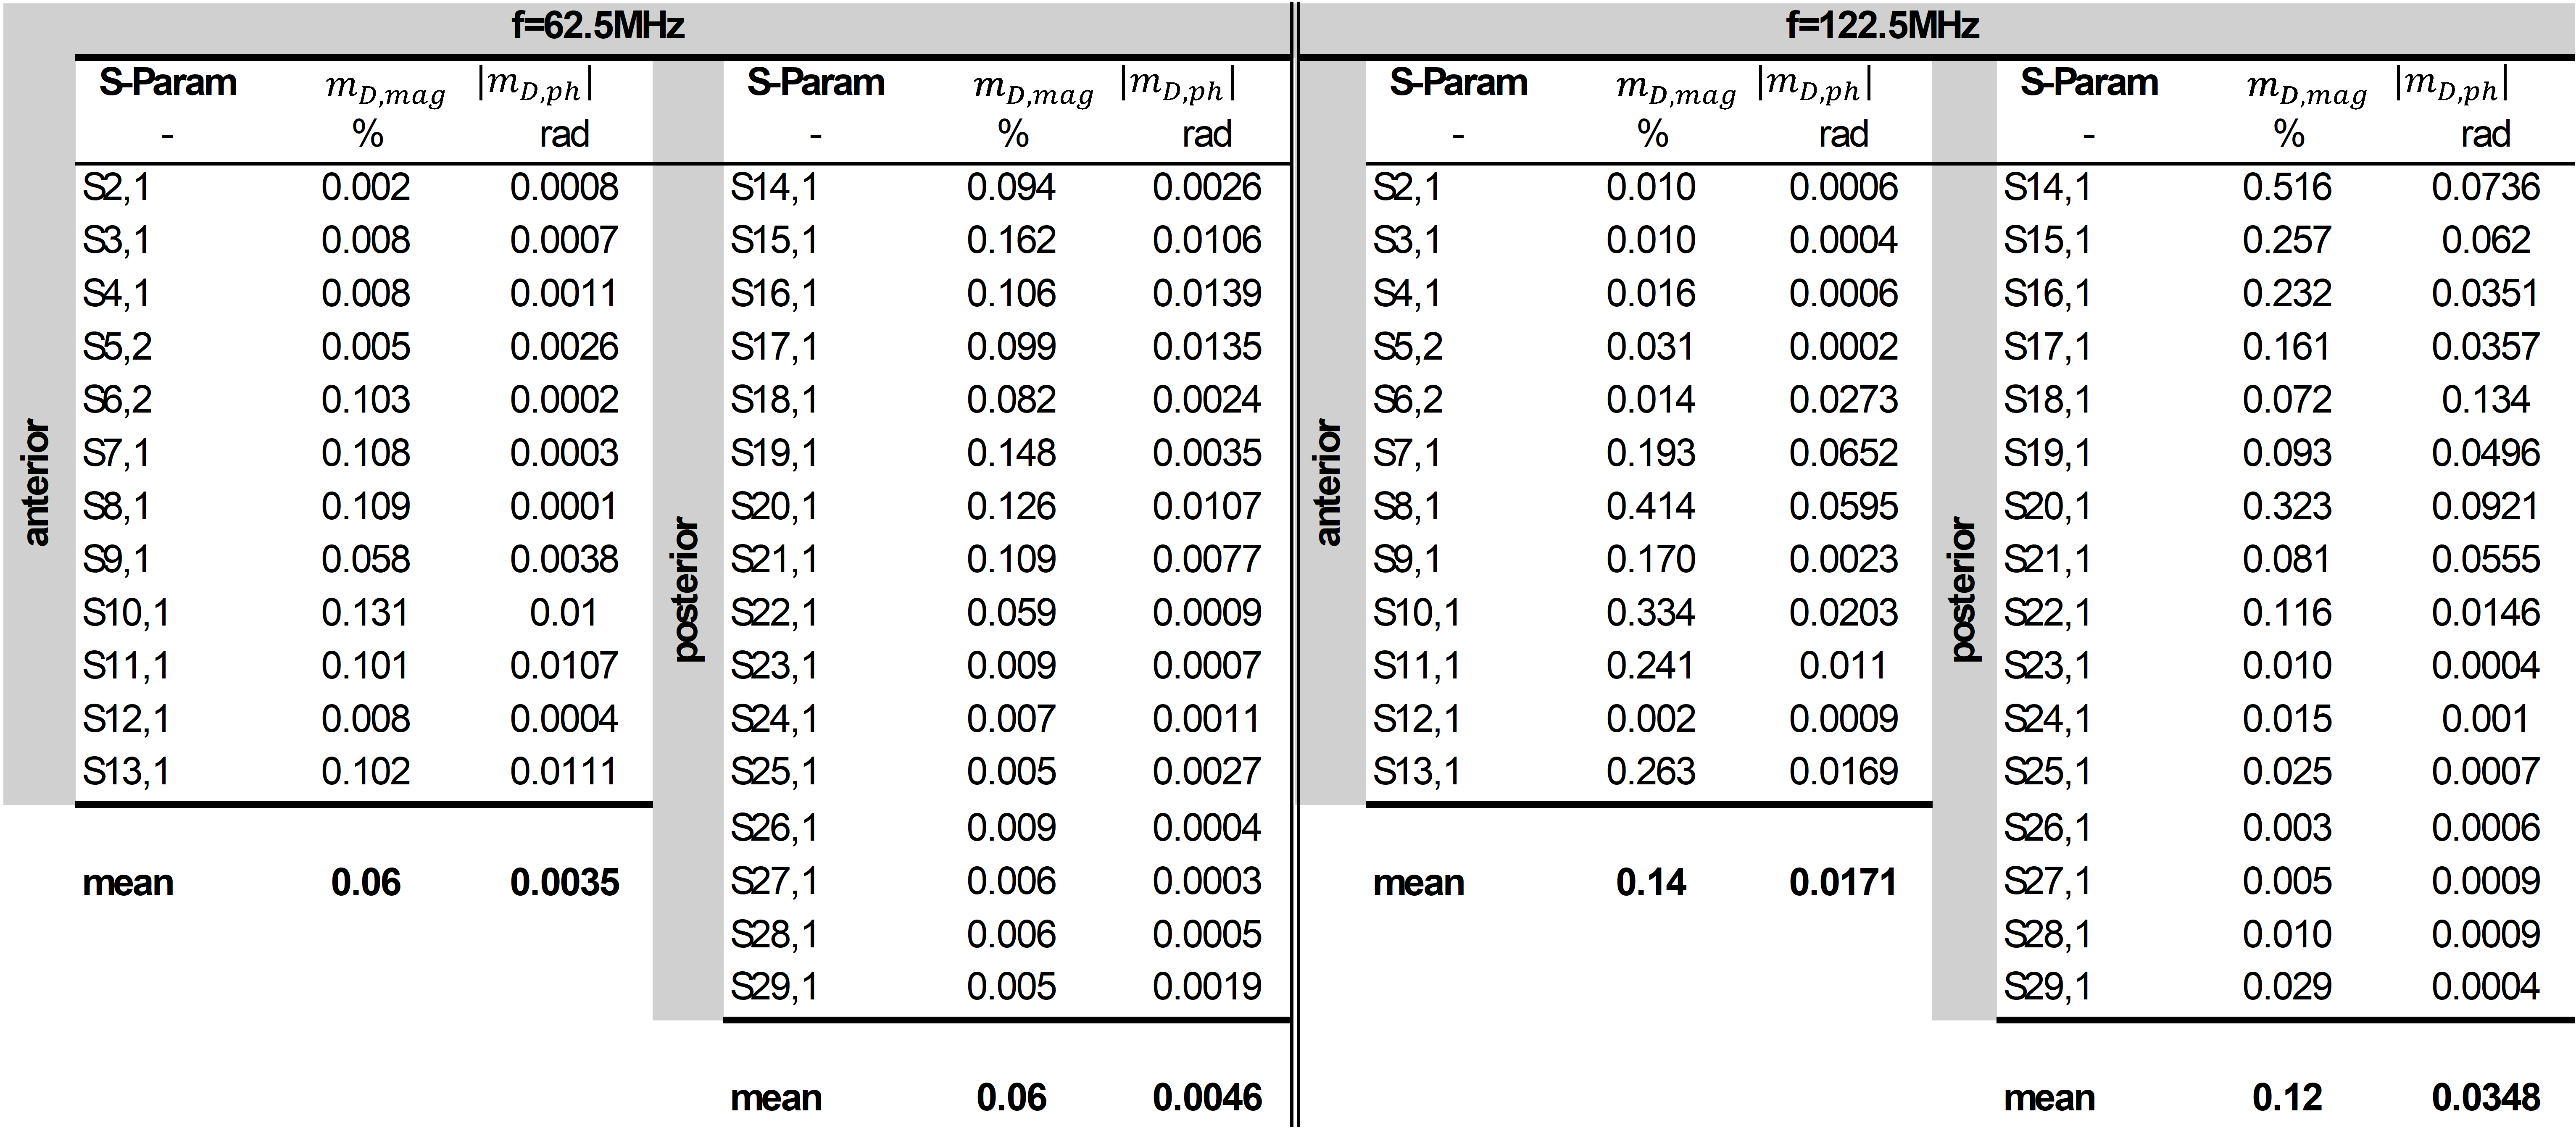
\includegraphics{./media/image10.png}
\caption{Magnitude (\(m_{D,mag}\)) and absolute phase (\(|m_{D,ph}|\))
modulation depths of all anterior and posterior elements at f=62.5MHz
and f=122.5MHz}
\label{fig:mod-depth-summary}
\end{figure}

% NOTE: .emf graphics aren’t supported by pdfLaTeX on Overleaf.
% Convert these to PDF/PNG (e.g., image11.png/image12.png) and re-enable.
%
%\begin{figure}
%\centering
%\includegraphics{./media/image11.png}
%\caption{Bar-graph of magnitude modulation depths in percent
%in anterior (top) and posterior (bottom) elements at f=62.5MHz and
%f=122.5MHz}
%\label{fig:mod-depth-bars-mag}
%\end{figure}
%
%\begin{figure}
%\centering
%\includegraphics{./media/image12.png}
%\caption{Bar-graph of phase modulation depths in radians in
%anterior (top) and posterior (bottom) elements at f=62.5MHz and
%f=122.5MHz}
%\label{fig:mod-depth-bars-phase}
%\end{figure}

\subsubsection{Modulation depth vs. PT
frequency}\label{modulation-depth-vs.-pt-frequency}

Evaluating modulation depth over the whole simulation frequency range of
10-150MHz revealed a strong dependence of transmission frequency and
position of the Rx coils with respect to the PT generator coil and the
phantoms heart.

Figure~\ref{fig:mod-depth-vs-frequency} shows absolute magnitude modulation depth (left) of all
channels over frequency, grouped by anterior (top) and posterior receive
elements (bottom). In general, modulation depths in the anterior array
tend to be lower than in the posterior array (0-0.75\% vs. 0-4\%). In
both plots, some channels have singular frequencies at which the
apparent absolute magnitude modulation is 0, indicating a geometric
situation similar to that described in Figure~\ref{fig:coupling-model}c where the sign of the
modulation changes and all modulation information is purely in the phase
data -- this behavior is especially prevalent in element S18,1.

Magnitude modulation increases approximately linearly with frequency in
the anterior elements.

In the posterior elements, magnitude modulation increases linearly up to
a frequency of around 130MHz, after which it starts to decrease.

Phase modulation increases strongly with frequency, both in the anterior
and posterior elements. Note that in Figure~\ref{fig:mod-depth-vs-frequency}, the dashed black line
shows mean \textbf{absolute} phase modulation.

\begin{figure}
\centering
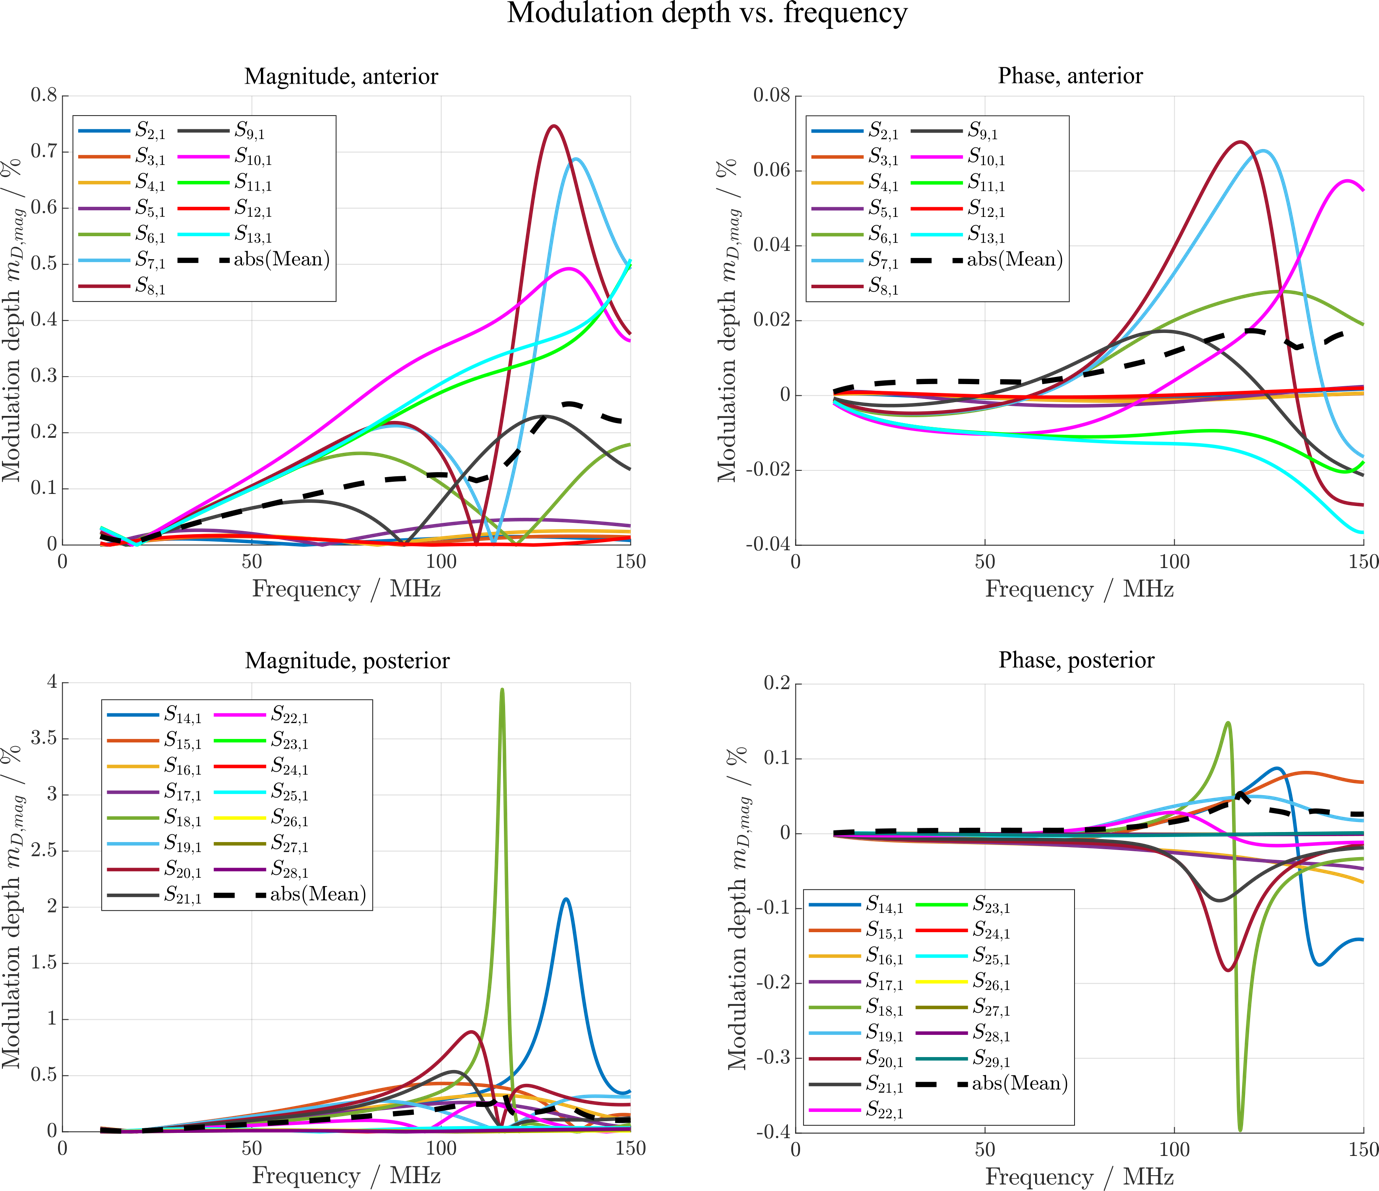
\includegraphics{./media/image13.png}
\caption{Calculated absolute magnitude (left) modulation
depth in percent and phase (right) modulation depth in radians for
anterior (top) and posterior (bottom) Rx channels. The dashed black line
shows the mean modulation depth over all channels. For phase, the dashed
black line shows mean \textbf{absolute} modulation depth.}
\label{fig:mod-depth-vs-frequency}
\end{figure}

\subsubsection{Per-channel correlation with cardiac volume}\label{per-channel-correlation}

\revgreen{Table~\ref{tab:per-channel} lists the signed Pearson correlation coefficient $R$ and modulation depth (Eqs.~\eqref{eq:mod-depth-mag} and~\eqref{eq:mod-depth-phase}) for each receive channel at both 62.5\,MHz and 122.5\,MHz, for both magnitude and phase. Channels where $|R| > 0.99$ exhibit near-perfect linear tracking of cardiac volume changes. Notably, most channels show $|R| > 0.97$ for both magnitude and phase, confirming that the PT signal can serve as a reliable surrogate for cardiac volume in nearly all spatial positions. Channel S2,1 at 62.5\,MHz and S12,1 at 122.5\,MHz show reduced magnitude correlation due to the sign-flip phenomenon discussed above, while phase correlation remains high in these channels.}

\begin{table}[ht]
\centering
\revred{
\caption{Per-channel signed Pearson correlation coefficient $R$ and modulation depth between the simulated S-parameter and heart volume ground truth. Magnitude modulation depth $m_{D,\text{mag}}$ is given in percent; phase modulation depth $m_{D,\text{ph}}$ in radians (signed, defined as the phase difference between maximum expansion and maximum contraction).}
\label{tab:per-channel}
\small
\begin{tabular}{l|rr|rr|rr|rr}
\hline
 & \multicolumn{4}{c|}{\textbf{62.5 MHz (1.5T)}} & \multicolumn{4}{c}{\textbf{122.5 MHz (3T)}} \\
 & \multicolumn{2}{c|}{Magnitude} & \multicolumn{2}{c|}{Phase} & \multicolumn{2}{c|}{Magnitude} & \multicolumn{2}{c}{Phase} \\
\textbf{Channel} & $R$ & $m_D$ [\%] & $R$ & $m_D$ [rad] & $R$ & $m_D$ [\%] & $R$ & $m_D$ [rad] \\
\hline
\multicolumn{9}{l}{\textit{Anterior array}} \\
\hline
$S_{2,1}$  & $+0.31$ & $0.02$ & $-0.99$ & $-0.001$ & $-1.00$ & $0.11$ & $+0.83$ & $+0.001$ \\
$S_{3,1}$  & $+1.00$ & $0.08$ & $-1.00$ & $-0.001$ & $-0.99$ & $0.10$ & $-0.94$ & $-0.000$ \\
$S_{4,1}$  & $+1.00$ & $0.08$ & $-1.00$ & $-0.001$ & $-0.99$ & $0.16$ & $-1.00$ & $-0.001$ \\
$S_{5,1}$  & $+1.00$ & $0.06$ & $-1.00$ & $-0.003$ & $-0.99$ & $0.34$ & $+0.98$ & $+0.000$ \\
$S_{6,1}$  & $-1.00$ & $1.38$ & $-0.92$ & $-0.000$ & $+0.97$ & $0.20$ & $+1.00$ & $+0.027$ \\
$S_{7,1}$  & $-1.00$ & $1.40$ & $-0.87$ & $-0.000$ & $+1.00$ & $2.84$ & $+1.00$ & $+0.065$ \\
$S_{8,1}$  & $-1.00$ & $1.42$ & $-0.03$ & $+0.000$ & $+1.00$ & $6.17$ & $+1.00$ & $+0.060$ \\
$S_{9,1}$  & $-1.00$ & $0.78$ & $+1.00$ & $+0.004$ & $+1.00$ & $2.46$ & $+1.00$ & $+0.002$ \\
$S_{10,1}$ & $-1.00$ & $1.70$ & $-1.00$ & $-0.010$ & $-1.00$ & $4.78$ & $+1.00$ & $+0.020$ \\
$S_{11,1}$ & $-1.00$ & $1.25$ & $-1.00$ & $-0.011$ & $-1.00$ & $3.25$ & $-1.00$ & $-0.011$ \\
$S_{12,1}$ & $+0.99$ & $0.08$ & $-0.99$ & $-0.000$ & $-0.36$ & $0.02$ & $+1.00$ & $+0.001$ \\
$S_{13,1}$ & $-1.00$ & $1.26$ & $-1.00$ & $-0.011$ & $-1.00$ & $3.53$ & $-1.00$ & $-0.017$ \\
\hline
\multicolumn{9}{l}{\textit{Posterior array}} \\
\hline
$S_{14,1}$ & $-1.00$ & $1.23$ & $-0.99$ & $-0.003$ & $-1.00$ & $7.88$ & $+1.00$ & $+0.074$ \\
$S_{15,1}$ & $-1.00$ & $2.16$ & $-1.00$ & $-0.011$ & $-1.00$ & $3.77$ & $+1.00$ & $+0.062$ \\
$S_{16,1}$ & $-1.00$ & $1.36$ & $-1.00$ & $-0.014$ & $-1.00$ & $3.26$ & $-1.00$ & $-0.035$ \\
$S_{17,1}$ & $-1.00$ & $1.25$ & $-1.00$ & $-0.014$ & $-1.00$ & $2.23$ & $-1.00$ & $-0.036$ \\
$S_{18,1}$ & $-1.00$ & $1.09$ & $-0.98$ & $-0.002$ & $+0.78$ & $1.15$ & $-1.00$ & $-0.134$ \\
$S_{19,1}$ & $-1.00$ & $2.09$ & $-0.99$ & $-0.004$ & $+1.00$ & $1.43$ & $+0.99$ & $+0.050$ \\
$S_{20,1}$ & $-1.00$ & $1.73$ & $-1.00$ & $-0.011$ & $+0.98$ & $5.14$ & $-1.00$ & $-0.092$ \\
$S_{21,1}$ & $-1.00$ & $1.49$ & $-0.99$ & $-0.008$ & $+0.87$ & $1.25$ & $-1.00$ & $-0.056$ \\
$S_{22,1}$ & $-1.00$ & $0.83$ & $+0.86$ & $+0.001$ & $+1.00$ & $1.79$ & $-0.99$ & $-0.015$ \\
$S_{23,1}$ & $+1.00$ & $0.08$ & $-1.00$ & $-0.001$ & $-1.00$ & $0.10$ & $-1.00$ & $-0.000$ \\
$S_{24,1}$ & $+0.99$ & $0.07$ & $-1.00$ & $-0.001$ & $-1.00$ & $0.14$ & $-0.99$ & $-0.001$ \\
$S_{25,1}$ & $+0.89$ & $0.05$ & $-1.00$ & $-0.003$ & $-1.00$ & $0.26$ & $-0.91$ & $-0.001$ \\
$S_{26,1}$ & $+1.00$ & $0.09$ & $-0.98$ & $-0.000$ & $-0.94$ & $0.03$ & $-0.96$ & $-0.001$ \\
$S_{27,1}$ & $+1.00$ & $0.05$ & $-0.99$ & $-0.000$ & $-0.97$ & $0.04$ & $-1.00$ & $-0.001$ \\
$S_{28,1}$ & $+1.00$ & $0.05$ & $-0.99$ & $-0.001$ & $-0.99$ & $0.09$ & $-1.00$ & $-0.001$ \\
$S_{29,1}$ & $+1.00$ & $0.05$ & $-1.00$ & $-0.002$ & $-0.99$ & $0.30$ & $-0.96$ & $-0.000$ \\
\hline
\end{tabular}
}
\end{table}

\subsection{Experimental S-parameter measurements}\label{experimental-results}

\begin{revbrownblock}

Table~\ref{tab:exp-sparams} summarises the measured scattering parameters and cardiac modulation depths for all three volunteers. The PT signal was detected in all active receive channels, with $S_{1,n}$ values ranging from $-79$ to $-120$\,dB across all subjects and channels.

\begin{table}[htbp]
\centering
\caption{Experimental S-parameter levels and cardiac modulation depths per volunteer. Modulation depth is defined as peak-to-peak excursion of the averaged cardiac waveform in $S_{1,n}$\,(dB). N\textsubscript{cycles} denotes the number of cardiac cycles averaged.}
\label{tab:exp-sparams}
\resizebox{\columnwidth}{!}{%
\begin{tabular}{lcccccccc}
\hline
 & \multicolumn{2}{c}{$S_{1,n}$ range (dB)} & \multicolumn{2}{c}{Mag.\ mod.\ depth (\%)} & \multicolumn{2}{c}{Phase mod.\ depth (\%)} & & \\
Volunteer & Anterior & Posterior & Ant.\ mean & Post.\ mean & Ant.\ mean & Post.\ mean & N\textsubscript{ch} & N\textsubscript{cycles} \\
\hline
V1 & $[-93, -118]$ & $[-118, -120]$ & 0.005 & 0.001 & 0.075 & 0.032 & 27 & 17 \\
V2 & $[-79, -119]$ & $[-111, -120]$ & 0.003 & 0.002 & 0.088 & 0.113 & 24 & 22 \\
V3 & $[-93, -118]$ & $[-117, -120]$ & 0.010 & 0.003 & 0.105 & 0.132 & 27 & 22 \\
\hline
\multicolumn{3}{l}{Pooled (all volunteers)} & 0.006 & 0.002 & 0.089 & 0.092 & 78 & --- \\
\hline
\end{tabular}
}
\end{table}

% [FIGURE PLACEHOLDER: Averaged cardiac waveforms for strongest channels, all 3 volunteers]
% \begin{figure}[htbp]
% \centering
% \includegraphics[width=\columnwidth]{./media/exp_waveforms.png}
% \caption{Averaged cardiac waveforms (magnitude and phase) for the three strongest anterior channels per volunteer. Shaded bands indicate 95\,\% CI from cycle averaging. [V1: 17 cycles, V2: 22 cycles, V3: 22 cycles]}
% \label{fig:exp-waveforms}
% \end{figure}

% [FIGURE PLACEHOLDER: Modulation depth bar chart per volunteer]
% \begin{figure}[htbp]
% \centering
% \includegraphics[width=\columnwidth]{./media/exp_moddepth_bar.png}
% \caption{Cardiac modulation depth ($S_{1,n}$\,dB) per channel for all three volunteers. Anterior channels (B\textit{xx}) shown in blue, posterior channels (S\textit{xx}) in orange.}
% \label{fig:exp-moddepth}
% \end{figure}

Anterior channels exhibited consistently stronger absolute coupling ($S_{1,n} \approx -93$ to $-118$\,dB) compared to posterior channels ($-111$ to $-120$\,dB), reflecting the closer proximity of the anterior array to the integrated PT generator. Notably, the strongest anterior channels (V1: B22, $-93$\,dB; V2: B24, $-79$\,dB; V3: B22, $-93$\,dB) receive PT signal levels approximately 25--40\,dB above the receiver noise floor of $-120$\,dBm. Even the weakest posterior channels, at approximately $-120$\,dB, remain at the boundary of the receiver's calibrated linear range.

Phase modulation depths were consistently an order of magnitude larger than magnitude modulation depths across all volunteers (pooled: 0.09\,\% phase vs.\ 0.005\,\% magnitude), mirroring the simulation finding that phase carries more cardiac information than magnitude for channels not directly aligned with the heart.

Posterior elements, despite their weaker absolute coupling, showed comparable or even larger phase modulation depths than anterior elements in V2 (0.113\,\% vs.\ 0.088\,\%) and V3 (0.132\,\% vs.\ 0.105\,\%). This is consistent with the simulation prediction of higher modulation depth in the transmissive geometry, where the heart lies on a direct path between generator and posterior receiver.

The inter-subject variability in $S_{1,n}$ levels and modulation depths reflects differences in body habitus (height, weight, subcutaneous fat thickness) and the resulting variation in generator-to-heart and heart-to-coil distances. Additionally, exact coil placement on the body surface --- which determines the spatial overlap between each element's sensitivity profile and the cardiac displacement volume --- differs between subjects and coil configurations (Body~18 vs.\ Body~12).

% [FIGURE PLACEHOLDER: Simulation vs. experimental comparison]
% \begin{figure}[htbp]
% \centering
% \includegraphics[width=\columnwidth]{./media/sim_vs_exp.png}
% \caption{Comparison of simulated and experimentally measured S-parameter modulation depths at 62.5\,MHz. Simulation values (12 anterior + 16 posterior channels) shown alongside experimental data (pooled across volunteers). Note the simulation represents an idealised upper bound without noise or receiver chain effects.}
% \label{fig:sim-vs-exp}
% \end{figure}
\end{revbrownblock}
Comparing to simulation: the simulated $S_{1,n}$ range at 62.5\,MHz was approximately $-54$ to $-95$\,dB (anterior S2--S13: $-60$ to $-82$\,dB; posterior S14--S29: $-72$ to $-95$\,dB), while measured values are 20--30\,dB weaker. This difference is expected: the simulation uses idealised port coupling ($50\,\Omega$ matched, no cable losses) and a single standardised body geometry, whereas the experiment includes cable attenuation, connector losses, impedance mismatches, and inter-subject anatomical variation. The simulated magnitude modulation depths (0.03--1.7\,\% at 62.5\,MHz) represent an upper bound; the measured values (0.001--0.07\,\%) are approximately one order of magnitude lower, consistent with the cumulative effect of receive chain losses and noise. Importantly, the qualitative spatial pattern --- stronger modulation in channels overlapping the heart, phase exceeding magnitude, posterior channels showing high modulation depth despite weak coupling --- is preserved in both simulation and experiment.

\section{Discussion}\label{discussion}

\rev{The simulation framework presented here demonstrates how
physiological motion leads to modulations of the Pilot Tone signal by
inductive coupling of the generator coil to the receiving coils via
conductive tissues.}

\revpink{The theoretical framework developed above --- from the volume integral formulation (Eq.~\ref{eq:vn-integral}) to the simplified equivalent circuit (Figure~\ref{fig:equivalent-circuit}) --- is intended to build intuitive understanding of the underlying physical principles. Since realistic human anatomy, with its heterogeneous, anisotropic tissue distribution and complex cardiac geometry, is far too complex to solve these equations analytically, the full-wave numerical simulation expands on the theory by solving Maxwell's equations on a discretised model without simplifying assumptions. Nevertheless, the analytical framework offers valuable qualitative insights that guide interpretation of both simulation and experimental results. For instance, the volume integral (Eq.~\ref{eq:vn-integral}) shows that signal modulation is governed by the admittivity-weighted field overlap: adipose tissue, with its comparatively low conductivity, does not significantly shield the PT signal but merely increases the source-to-coil distance --- predicting no fundamental degradation of PT performance in overweight patients, though a decrease in SNR is observed experimentally due to greater separation \cite{Bacher2017CardiacStudy}. Similarly, the theory predicts that coil placement is critical: the sensitivity of each receive channel depends on the spatial overlap between its electric field pattern and the cardiac displacement volume, explaining the wide variation in modulation depth across individual coils. Furthermore, the admittivity $\gamma = \sigma + j\omega\varepsilon$ suggests that signal strength scales with frequency through the permittivity term, and the superposition principle underlying the model explains why each coil receives a distinct mixture of respiratory, cardiac and other motion components --- the physical basis for separating these contributions through blind source separation methods \cite{Bacher2020PerformanceFramework}.}

\subsection{Noise and detectability}\label{noise-detectability}

The experimentally measured cardiac modulation depths (0.001--0.07\,\% in magnitude, 0.002--0.95\,\% in phase) are extremely small in absolute terms, raising the question of practical detectability. Two key factors enable reliable real-time cardiac signal extraction despite these low modulation depths. First, the receiver operates within an 85\,dB calibrated linear range ($-120$ to $-35$\,dBm); the measured PT levels ($-79$ to $-120$\,dB $S_{1,n}$) fall comfortably within this range, ensuring that the modulation is not obscured by receiver nonlinearity or quantisation noise. The received levels occupy approximately 27--40\,dB of the available dynamic range in the strongest channels, leaving substantial headroom.

Second, the real-time processing pipeline provides implicit and explicit noise suppression. The linear combination of multiple receive channels --- used to separate cardiac from respiratory motion components via blind source separation methods \cite{Bacher2020PerformanceFramework, BacherRetrospectiveCohort} --- inherently improves SNR by coherently combining cardiac signal from many elements while incoherent noise averages down. Subsequently, Kalman filtering in the temporal domain provides further explicit noise reduction, enabling robust cardiac trigger detection even in single-beat operation without the need for cycle averaging \cite{Bacher2022RobustPlacement, Bacher2021ProspectiveCine, Bacher2017CardiacStudy}. In the present validation experiment, cycle averaging over 17--22 heartbeats was employed solely to characterise the noise floor and demonstrate signal quality --- this step is not required in the real-time processing chain.

The simulation, which includes no noise sources, receiver imperfections, or cable losses, represents an idealised upper bound: simulated modulation depths are approximately one order of magnitude larger than measured values. This is consistent with the cumulative attenuation of the receive chain (estimated at 20--30\,dB from the $S_{1,n}$ level comparison). Crucially, however, the spatial patterns of modulation are preserved: channels with strong simulated cardiac sensitivity also show strong experimental modulation, phase consistently dominates over magnitude, and posterior elements exhibit high modulation depth despite weak absolute coupling. The simulation thus correctly predicts \emph{which} channels carry cardiac information and the \emph{relative} modulation behaviour, while the \emph{absolute} levels are subject to the experimental receive chain attenuation.

The inter-subject variability (factor $\sim$2--3 in modulation depth between volunteers) is attributable to differences in body habitus --- particularly thorax depth, subcutaneous fat layer thickness, and heart-to-array distance --- as well as variation in exact coil placement on the body surface. This is directly predicted by the volume integral formulation (Eq.~\ref{eq:vn-integral}): both the generator field $\mathbf{E}_1$ and receiver sensitivity $\mathbf{E}_n$ decay with distance, such that larger source-to-heart or heart-to-coil separations reduce the overlap integral and thus the modulation depth.

\subsection{Variations in conductivity and
permittivity}\label{variations-in-conductivity-and-permittivity}

The illuminated area of each receiving coil is relatively small compared
to the whole body and therefore the signal modulation in each coil is
somewhat localized, with each individual coil receiving only motion
modulation stemming from within its field of view. We argue that the
measured signal modulation in each coil can be explained by gradual
replacement of tissues within the area illuminated by both receiver and
generator. Consider the case of diaphragmatic motion during expiration,
where the diaphragm shifts upwards and lung tissue is displaced by,
mainly, liver tissue: Over the course of a respiratory cycle, a receive
coil lying anterior to the diaphragm would see the amount of liver
tissue (low conductivity and permittivity) increase, while the amount of
lung tissue (higher conductivity and permittivity) decreases and vice
versa. Consequently, the bulk conductivity and permittivity, in the
illuminated area changes and thus modulates the received signal.

Several other tissue types have interesting properties that are
beneficial to this method: Bone and fat for instance have extremely low
conductivity and permittivity. This is fortunate, as eddy currents in
fat and bone are negligible and do not significantly weaken the magnetic
field. We have previously observed that high BMI does not significantly
attenuate the received signal \cite{Bacher2017CardiacStudy}.

Similarly, blood and myocardium differ significantly in their respective
properties, especially conductivity and by this two-compartment tissue
replacement model should, and in practice do, yield high signal
modulation, advancing the hypothesis that PT may provide a valuable
alternative to the ECG or MRI-derived signals used for gating,
triggering, or binning \cite{Qian2025ComparisonStudy, Mizuno2024ClinicalLeads}.

\subsection{\texorpdfstring{Virtual human
}{Virtual human }}\label{virtual-human}

Simulation results on the virtual human model show similar signal
features as seen in vivo: In vivo, cardiac signal is present in most
channels, even those that are relatively far away from the heart.
According to the simulation, signal modulation correlated to cardiac
motion is to be expected in all coils. This behavior is consistent with
in-vivo experiments, where channels far away from the heart often carry
significant cardiac signal \cite{Bacher2017PilotInitialization, Bacher2017CardiacStudy}. The modulation depth in our
simulations is similar to those found in vivo, around 0.03 percent on
average at 1.5T \cite{Bacher2017CardiacStudy}.

Modulation depth was higher overall in the posterior elements. This is
due to the more ideal geometry, where the heart lies, for most channels,
on a straight path between the generator loop (primary side) and Rx loop
(secondary side) -- in this case the measurement is more
``transmissive'', similar to the experiments made by Moskalenko et al. -
though we would discourage the use of this term at such low frequencies.

In practice, a cardiac signal component is sometimes not discernible in
very far away channels, where both direct coupling and modulation depth
are low due to distance and signal modulation can be below the noise
floor. Especially in posterior channels the cardiac signal modulation is
often too weak compared to the receivers noisefloor, because these
channels are much further away from the PT generator and, crucially,
from the eddy currents and the secondary field generated in the heart
and thus the source of the signal modulation.

Note the weak correlation in channel S2,1 in Figure~\ref{fig:rx-magnitude-62} -- here the signal
shows clear dependence on simulated cardiac volume but appears to
``flip'' sign during the cardiac cycle.

This is likely due to geometries similar to the case presented in Figure~\ref{fig:coupling-model}, where at certain points in space the secondary fields generated by
eddy currents from different conducting domains cancel each other out,
magnitude modulation in this point is zero and either positive or
negative in the space around this point. Phase modulation however, is
still present in these areas. An example of this behavior is channel
S2,1 at 62.5MHz where correlation to cardiac volume is very weak in the
magnitude signal (Figure~\ref{fig:rx-magnitude-62}) but excellent in the phase signal (Figure~\ref{fig:rx-phase-62})
or S12,1 at 122.5MHz (Figures~\ref{fig:rx-magnitude-122} and~\ref{fig:rx-phase-122}).

This behavior can also be observed in the modulation depth vs. frequency
analysis: Element S18,1 at 120.6MHz for instance shows zero magnitude
modulation but strong phase modulation of -0.19 radians.

These results suggest that complex valued processing of PT data can
avoid ``blind spots'' in sensitivity to motion that can occur in
magnitude only processing.

The strong correlation of the received signal with cardiac volume ground
truth \revred{($|R| > 0.94$ on average across all channels and both frequencies, Table~\ref{tab:correlation})} suggests that, at least approximately, the cardiac PT signal may
be seen as a proxy for total cardiac volume. Importantly, maxima and
minima of the heart volume curve (i.e. the onset of mechanical systole
and the point of maximum contraction) closely match ground truth.

As the generated field is not homogeneous, falling off with distance
cubed, motion closer to the generator will contribute more to the
received signal than motion further away. It is therefore crucial for
best performance to position the PT field generator loop as close to the
heart as possible, though some centimeters of tolerance are acceptable.
When integrating the PT generator in e.g. a abdominal coil array, it
must be designed in such a way that the generator is optimally located
when the coil array is positioned for optimal imaging.

\subsubsection{\rev{Generator placement}}\label{generator-placement}

\rev{The position of the PT generator coil relative to the heart is a key design parameter. In this work, the generator was placed anterior to the chest wall, directly above the heart, consistent with practical implementations where the PT source is integrated into the anterior coil array housing. Because the primary magnetic field decays with $r^{3}$ (magnetic dipole), the induced eddy currents and consequently the secondary field scale strongly with distance. A generator placed closer to the heart produces stronger tissue-mediated coupling and thus higher modulation depths, while a more distant placement yields more uniform illumination at the expense of sensitivity. Optimization of generator position for specific clinical applications remains an interesting topic for future work.}

\subsubsection{Limitations of the model}\label{limitations-of-the-model}`

While in vivo results agree well with simulations, some factors were not
modeled: The received signal is subjected to an extensive and complex
processing chain: Amplification, demodulation, digital sampling,
switching etc. and component non-idealities were not considered in this
simulation and neither were the physical characteristics of the coils
themselves, i.e. geometric properties such as overlap and electric
properties like impedances. Especially the noise characteristics of the
analog receiver does impose limits on the reception of these extremely
weak signals and in practice not all Rx elements have sufficient signal
to noise ratio, especially those farthest away from the PT generator
loop.

These simulations should therefore be taken as a upper bound for
received signal modulation as corroborated by our results.

Also, an extension to higher frequencies, e.g. to 300MHz for 7T systems
proved infeasible due to computational demand, at least with the
simulation setup used in this work. Methods like those proposed by
Jaeschke et al. (42-44) at 7T or Anand et al. (8, 56, 75) at 1.5/3T but
using low GHz range carriers are an interesting target for further
simulation studies.

\revturquoise{While the frequency-domain solver provides broadband S-parameter data through Gaussian pulse excitation (Figure~\ref{fig:mod-depth-vs-frequency}), several aspects of the practical receive system are not captured in the simulation. Coil tuning was not modeled: the receive elements were treated as ideal ports without matching networks, whereas in practice each element has a bandpass response centered at the Larmor frequency. 
Since the PT carrier is chosen close to, but not exactly at, the Larmor frequency, the receive sensitivity at $f_{PT}$ is reduced but not prohibitively attenuated. Furthermore, coil geometry was kept constant across the frequency sweep, whereas different field strengths employ different array designs with adapted element sizes. Patient-dependent detuning from body loading, the frequency-dependent gain and phase response of the downstream receive chain (preamplifiers, cables, baluns), and mutual coupling between array elements were likewise not modeled.}

\revturquoise{These limitations primarily affect the absolute received signal levels but do not alter the underlying modulation mechanism. The broadband S-parameter data confirms that the physical principles --- admittivity-weighted field overlap, spatial sensitivity dependence, and superposition of motion components --- operate consistently across the simulated bandwidth and produce qualitatively identical behaviour at both 62.5 and 122.5\,MHz. The simulation thus represents an idealised upper bound for modulation depth. Actual values will be lower due to receive chain imperfections and noise.}

\revturquoise{The volume integral formulation offers insight into the expected frequency scaling: induced electric fields scale as $E \propto \omega$ (Faraday's law) while direct inductive coupling scales identically, yielding a body-mediated modulation depth that increases approximately linearly with frequency. This has direct implications at the extremes of current clinical field strengths. At 0.55\,T ($f_{PT} \approx 23$\,MHz), the model predicts modulation depths roughly $3\times$ lower than at 1.5\,T --- consistent with the observation by Tasdelen et al.\ that cardiac PT gating at 0.55\,T requires substantially increased transmit amplitude to achieve detectable cardiac signals, and that no successful cardiac PT gating at field strengths below 1.5\,T had been demonstrated prior to their work \textcolor{red}{\cite{Tasdelen2025HAPTIC}}. At 7\,T, Jaeschke et al.\ demonstrated that cardiac motion modulates the scattering parameters of an RF transmit array, confirming that the coupling mechanism strengthens at higher frequency as predicted \textcolor{red}{\cite{Jaeschke2018Cardiac7T}}. However, at 7\,T the PT frequency approaches the bore waveguide cutoff, potentially transitioning from the evanescent to the propagating regime and introducing wave-interference effects not captured by the quasi-static model. Dedicated simulations at both 0.55\,T and 7\,T, incorporating field-strength-appropriate coil geometries and accounting for potential near-field breakdown at ultra-high field, represent an interesting direction for future work.}

As for physiology, the electromagnetic parameters in tissue were modeled
isotropic, whereas in reality, most tissues exhibit strong anisotropy.
Muscle fibers for instance are much more conductive in axial (1S/m) than
radial (0.2S/m) direction \cite{Beck2005AAmplitudes}. To our knowledge, no commercial
solvers currently exist that support tensorial electromagnetic
parameters throughout the numerical simulation.
\rev{However, the isotropic approximation is standard practice in RF safety simulations and MRI coil modeling at clinical frequencies. The bulk effect of tissue redistribution during cardiac motion (replacing one tissue type with another) is expected to dominate over local anisotropy effects. Furthermore, the volume-integrated nature of the PT signal (Appendix, Eq.~\ref{PortVoltage}) averages over many fiber orientations, reducing the impact of directional conductivity variations on the net modulation depth.}


\revorange{Respiratory motion was not included in the present simulation framework. Unlike cardiac motion, which modulates the PT signal exclusively through redistribution of tissue admittivity within the illuminated volume (Eq.~\ref{eq:vn-integral}), respiration additionally displaces the PT transmit coil itself, typically mounted on or integrated into the anterior array, along with the chest wall. This geometric displacement of the source directly changes the field patterns $\mathbf{E}_1$ and consequently the coupling to all receive elements, producing modulation depths one to two orders of magnitude larger than the cardiac signal. Schroeder et al.\ \cite{Schroeder2016a} demonstrated that two respiratory components, related to chest-wall motion (chest breathing) and internal tissue displacement (e.g.\ liver, abdominal breathing), can be separated and independently characterized. This large modulation depth that makes respiratory PT navigation comparatively straightforward \cite{Speier2015PT-Nav:MR-receiver, Vahle2020RespiratoryTone, Rigie2018TrackingNavigation, Lenk2018RespiratoryTechnology, Schroeder2016a}. The cardiac case, where the signal arises solely from the tissue-replacement mechanism at considerably smaller modulation depths, represents the more instructive and technically challenging scenario and is therefore the focus of this work.}

\section{Conclusion}\label{conclusion-1}

We proposed a theoretical model for the Pilot Tone navigator and
performed numerical simulations to \rev{investigate} the physical processes
resulting in the received, motion modulated Pilot Tone signal.

We then demonstrated how receive coils placed around the abdomen receive
signals modulated by physiological organ motion and that these signals
differ in their sign, modulation depth and correlation to cardiac motion
and were able to confirm that the received signals correlate closely to
total cardiac volume.

We further showed how PT frequency influences the received signal and
found that in the frequency range used by clinical MRI scanners a stable
signal can be obtained in most receive coil elements.

\subsection{Outlook}\label{outlook}

This direct relation allows for triggering or gating to the actual
motion of the heart. The high temporal resolution and continuous
sampling of the PT signal may also allow for identification of other
interesting features, e.g. the end of systole (point of maximum
contraction -- the minimum in the cardiac PT signal), a point that is
not easily inferred from the distorted ECG available in a clinical MRI
scanner.

In these simulations, we concentrated on the cardiac signal but using
the XCat phantom, respiratory and even combined respiratory and cardiac
simulations are possible. Our simulations may easily be expanded to
investigate the effect of respiratory motion or even motion of other
body parts, possibly even that of the head \cite{Speier2018SeparationMeasurements}. During respiration,
in a typical MRI exam, the anterior coil array will move with the chest
and abdomen, thus creating significant signal modulation simply due to
the change in distance between PT generator loop and Rx elements. The
simulation presented here is comparable to a breathheld exam.

As the PT carrier frequency needs to be close to the proton resonance
frequency, it is constrained by the system's field strength. Overall,
modulation depth both in magnitude and phase benefits from moving to
higher frequencies. While Pilot Tone has been implemented by us on 0.55T
systems, it is currently only used for respiration. Extracting a stable
cardiac signal is challenging, because modulation depths at this
frequency are low compared to 3T or even 1.5T, though Tasdelen et al.
\cite{Tasdelen2025ContactlessHAPTIC} recently showed that retrospective gating is feasible by using
a higher powered carrier signal and careful signal separation.

At 7T, Jaeschke et al. \cite{Jaeschke2017, Jaeschke2017a, Jaeschke2019ScatteringMonitoring} demonstrated a method based on the
same physical principles, utilizing direct measurements of the S-matrix.

Different carrier frequencies do, however, result in different field
distributions. In the future, we believe that investigations into using
different or multiple simultaneous PT frequencies could improve
performance.

Finally, it is worth noting that PT can be implemented at relatively
little cost on, theoretically, any MR system and enables continuous,
sequence independent respiratory and cardiac motion monitoring at very
high temporal resolution and without the need for ECG, navigators or
respiratory bellows. Processing of PT motion data \cite{Bacher2017CardiacStudy, Bacher2020PerformanceFramework} is
decoupled from sequence execution, allowing flexible sequence design.
Gradient or magnetohydrodynamic artefacts, often encountered in ECG,
especially at field strengths \textgreater1.5T are avoided. Also, no
patient preparation is necessary, potentially saving time in clinical
environments while particular expertise in ECG lead placement especially
at higher field strength may no longer be needed. We have demonstrated
here that the underlying physical principles work on a broad range of
frequencies and in all patients.

\subsection{Author's contribution
statement}\label{authors-contribution-statement}

Conceptualization and methodology, theoretical model: Mario Bacher and
Peter Speier

Numerical simulations and data analysis: Mario Bacher

Writing of original draft: Mario Bacher

Writing, review and editing: Mario Bacher, Peter Speier, Matthias Stuber

Project supervision: Matthias Stuber

All authors contributed to the interpretation of results and approved
the final manuscript.

\subsection{Conflicts of interest}\label{conflicts-of-interest}

Mario Bacher and Peter Speier are employees of Siemens Healthineers AG.

\subsection{Funding statement}\label{funding-statement}

No external funding was received for this work.

\subsection{Data Availability
Statement}\label{data-availability-statement}

The XCat virtual phantom data used to generate the data for this study
was used under license from the Center For Virtual Imaging Trials, Duke
University (https://cvit.duke.edu/resource/xcat-phantom-program/) and so
cannot be made freely available. The simulation results used to support
the findings of this study are available from the corresponding author
upon request.



\printbibliography

\appendix
% --- APPENDIX ---
\section{Assumptions}
\label{app:derivation}
% Full Maxwell → Reciprocity → V_n derivation
% Born approximation formal conditions
% RLC parameter extraction
% S-parameter network theory

The electromagnetic environment is modeled as a time-harmonic system at the PT frequency ($f_{PT}=62.5MHz$ at $1.5T$ and $f_{PT}=122.5MHz$ at 3T) with $\omega=2\pi f_{PT}$.

Maxwells curl equations in the source region are:

\begin{align}
    \nabla \times \mathbf{E} = -j\omega\mu_0 \mathbf{H} \label{maxwell1}\\
    \nabla \times \mathbf{H} = \mathbf{J}_{src} + (\sigma+j\omega\epsilon)\mathbf{E} \label{maxwell2}
\end{align}

where $\mathbf{J}_{src}$ is the current density in the transmit loop (zero elsewhere), $\sigma$ is the electrical conductivity, $\epsilon$ is the permittivity and $\mu_0$ is the permeability of free space.

To simplify the derivation, we make the following assumptions:
\begin{itemize}
    \item all media are linear and \rev{isotropic}
    \item all media are non-magnetic, i.e. relative permeability is $\mu_r=1$ everywhere so that $\mathbf{B}=\mu_0 \mathbf{H}$
    \item the system is in a steady-state at frequency $\omega$. Transient motion effects are ignored as the time scale is orders of magnitude lower.
    \item Tissue properties are real-valued everywhere. We use complex admittivity defined as $\gamma = \sigma + j\omega\epsilon$
\end{itemize}

\section{Lorentz Reciprocity Theorem}

Consider two distinct electromagnetic configurations (a) and (b) applied to the same electromagnetic environment (same $\sigma(\rev{\mathbf{r}}), \epsilon(\rev{\mathbf{r}})$ and $\mu_0$), each with its own source and fields:

Configuration (a): source $\mathbf{J}^a$ on the loop conductor, zero elsewhere and fields $\mathbf{E}^a$ and $\mathbf{H}^a$

Configuration (b): source $\mathbf{J}^b$ and fields $\mathbf{E}^b$ and $\mathbf{H}^b$

We now seek to describe the Lorentz reciprocity identity

\begin{align}
    \label{lorentzreciprocity}
    \rev{\nabla \cdot} (\mathbf{E}^a \times \mathbf{H}^b - \mathbf{E}^b \times \mathbf{H}^a) = \rev{\nabla \cdot}(\mathbf{E}^a \times \mathbf{H}^b) - \rev{\nabla \cdot}(\mathbf{E}^b \times \mathbf{H}^a)
\end{align}

in terms of only sources and material parameters:

Using the product rule on the first term of \eqref{lorentzreciprocity}

\begin{align}
    \rev{\nabla \cdot}(\mathbf{E}^a \times \mathbf{H}^b) = \mathbf{H}^b \rev{\cdot} (\nabla \times \mathbf{E}^a) - \mathbf{E}^a \rev{\cdot} (\nabla \times \mathbf{H}^b)
\end{align}

Substituting Eq.\eqref{maxwell1} and Eq.\eqref{maxwell2} and using complex admittivity we arrive at 

\begin{align}
    \rev{\nabla \cdot}(\mathbf{E}^a \times \mathbf{H}^b) = \mathbf{H}^b \rev{\cdot} (-j \omega \mu_0 \mathbf{H}^a) - \mathbf{E}^a \rev{\cdot} (\mathbf{J}^b + \gamma \mathbf{E}^b) \\
    = -j \omega \mu_0 (\mathbf{H}^b \rev{\cdot} \mathbf{H}^a) - \mathbf{E}^a \rev{\cdot} \mathbf{J}^b - \gamma(\mathbf{E}^a \rev{\cdot} \mathbf{E}^b)
\end{align}

\rev{Similarly} for the second term of Eq.\eqref{lorentzreciprocity} we get

\begin{align}
    \rev{\nabla \cdot}(\mathbf{E}^b \times \mathbf{H}^a) = -j \omega \mu_0 (\mathbf{H}^a \rev{\cdot} \mathbf{H}^b) - \mathbf{E}^b \rev{\cdot} \mathbf{J}^a - \gamma(\mathbf{E}^b \rev{\cdot} \mathbf{E}^a)
\end{align}

Equation \eqref{lorentzreciprocity} is the difference of these two divergences:

Collecting term by term 
\begin{align}
    -j\omega\mu_0 (\mathbf{H}^a \rev{\cdot} \mathbf{H}^b) - (-j \omega \mu_0 (\mathbf{H}^a \rev{\cdot} \mathbf{H}^b)) = 0 \\
    -\gamma (\mathbf{E}^a \rev{\cdot} \mathbf{E}^b) - (-\gamma (\mathbf{E}^b \rev{\cdot} \mathbf{E}^a)) = -\gamma (\mathbf{E}^a \rev{\cdot} \mathbf{E}^b) +\gamma (\mathbf{E}^a \rev{\cdot} \mathbf{E}^b) = 0 \\
    -\mathbf{E}^a \rev{\cdot} \mathbf{J}^{\rev{b}} -(-\mathbf{E}^b \rev{\cdot} \mathbf{J}^a) = \mathbf{E}^b \rev{\cdot} \mathbf{J}^a - \mathbf{E}^a \rev{\cdot} \mathbf{J}^b
\end{align}

only $\mathbf{E}^b \rev{\cdot} \mathbf{J}^a - \mathbf{E}^a \rev{\cdot} \mathbf{J}^b$ remains and 

\begin{align}
\label{before_reciprocity}
    \rev{\nabla \cdot} (\mathbf{E}^a \times \mathbf{H}^b - \mathbf{E}^b \times \mathbf{H}^a) = \mathbf{E}^b \rev{\cdot} \mathbf{J}^a - \mathbf{E}^a \rev{\cdot} \mathbf{J}^b
\end{align}

Note that these cancellations require the above assumptions/simplifications that all tissue characteristics are \rev{isotropic} (scalar $\sigma$, $\epsilon$ $\rightarrow$ symmetric $\gamma$) and nonmagnetic (uniform $\mu_0$).

Integrating Eq. \eqref{before_reciprocity} over a volume $V$ bounded by a closed surface $S$ we find 

\begin{align}
    \label{reciprocity}
    \oiiint_{S} (\mathbf{E}^a \times \mathbf{H}^b - \mathbf{E}^b \times \mathbf{H}^a) \rev{\cdot} dS = \iiint_{V} (\mathbf{E}^b \rev{\cdot} \mathbf{J}^a - \mathbf{E}^a \rev{\cdot} \mathbf{J}^b) dV
\end{align}

the general Lorentz reciprocity theorem for lossy, dispersive, isotropic media. (Harrington 1961, Hoult 2000)

At port n, the fields on the cross section can be expressed in terms of port voltage $V_p$ and port current $I_p$ via the transmission line mode (citation pending):

\begin{align}
    \label{harringtonTLM}
    \int_{port \quad p}(\mathbf{E}^a \times \mathbf{H}^b - \mathbf{E}^b \times \mathbf{H}^a)dS = V_p^a I_p^b - V_p^b I_p^a
\end{align}

Summing over all N+1 ports:

\begin{align}
    \sum_{p=0}^{N} [V_p^a I_p^b -V_p^b I_p^a] = 0
\end{align}

For a two-port subset, where port 1 is driven in configuration a, port n is driven in configuration b, all other ports terminated we get:

\begin{align}
    V_1^a I_1^b + V_n^a I_n^b = V_1^b I_1^a + V_n^b I_n^a
\end{align}

In configuration a, port n is terminated (load $Z_0$ only, \rev{no} source) so the voltage at port n is purely due to coupling $ \rightarrow V_n^a = $ \rev{received} voltage from PT. In configuration b, port 1 is terminated, so $V_1^b =$ \rev{received} voltage from driven coil n.

For matched terminations and equal drive levels this yields the standard result:

\begin{align}
    \label{PortReciprocity}
    \frac{V_n^a}{I_1^a} = \frac{V_1^b}{I_n^b} \equiv Z_{n,1}
\end{align}

wherein $Z_{n,1}$ is the \rev{transimpedance} between port 1 and port n.


\subsection{Evaluation of the surface integral}

We apply the reciprocity Theorem (Eq. \eqref{lorentzreciprocity}) to the PT system, where configuration (a) is the PT transmitter as port $1$ and configuration (b) is the \rev{receive} element $n$. For a linear, isotropic system, the multi-port network is reciprocal ($Z_{n,1}=Z_{1,n}$).

We now derive the explicit expression for $V_n^a$, the voltage induced at receive port n by the PT transmitter.

We use Eq. \eqref{lorentzreciprocity} and \rev{separate} the volume integral into three non-overlapping regions: $V = V_{ports} \cup V_{body} \cup V_{free}$ where $V_{ports}$ contains the antenna conductors, $V_{body}$ is the tissue volume and $V_{free}$ is free space.

\rev{In} $V_{free}$\rev{:} $\sigma=0$, $\epsilon = \epsilon_0$ \rev{and there are no sources} $\rightarrow$ no contribution to the right side.

In $V_{ports}$ the source contribution is captured by the port terms of Eq. \eqref{harringtonTLM}. In $V_{body}$ there are no impressed sources ($\mathbf{J}^a=\mathbf{J}^b=0$, but $\gamma \neq 0$ since tissue has nonzero $\sigma, \epsilon$.

Splitting the integration volume allows us to rewrite the reciprocity theorem:

In the body volume there are no impressed sources, so
\begin{align}
    \label{Vbody}
    \oint_{S_{body}}(\mathbf{E}^a \times \mathbf{H}^b - \mathbf{E}^b \times \rev{\mathbf{H}}^a)\rev{\cdot}dS = 0
\end{align}

This states that the reciprocity surface integral vanishes over any surface enclosing only passive media - a well known result (citation pending).

To extract $V_n$ we use a different approach. The voltage at a terminated port can be written as \cite{Rumsey1954ReactionTheory}

\begin{align}
    \label{RumseyVoltage}
    \rev{\langle a,b \rangle} = \rev{\iiint}_V (\mathbf{E}^a \rev{\cdot} \mathbf{J}^b) dV
\end{align}

where $\rev{\langle a,b \rangle}$ is the "reaction", i.e. the response produced by the fields of configuration $a$ \rev{on} the sources of configuration $b$.

In tissue, we defined $\mathbf{J}^b=\gamma \mathbf{E}^b$ as the induced current.
According to \cite{Rumsey1954ReactionTheory} the port observable at port $n$ is simply the product of port voltage and port current $\rev{\langle a,b \rangle}=V_n I_n$ and with current normalized to $I_n=1A$ Eq. \eqref{RumseyVoltage} over the Volume $V_{body}$ is therefore

\begin{align}
    \label{PortVoltage}
    V_n = \iiint_{V_{body}} \mathbf{E}^a \rev{\cdot} \mathbf{J}^b dV \\
    V_n = \iiint_{V_{body}} \gamma (\mathbf{E}^a \rev{\cdot} \mathbf{E}^b) dV
\end{align}

This equation states that the received voltage at port $n$ $V_n$ equals the volume integral of the tissue admittivity $\gamma$ weighted by the overlap of the transmitter and receiver electric field - the coils sensitivity profile.

\subsection{Origin of the electric fields in electrically small source}

\rev{Henceforth we identify configuration (a) with the PT source (port 1) and configuration (b) with receive element n, writing $\mathbf{E}_1 \equiv \mathbf{E}^a$ and $\mathbf{E}_n \equiv \mathbf{E}^b$.}

The PT loop antennas size ($d=30mm$ in our simulations) is electrically small compared to the wavelength. The electrical size parameter is defined as $ka$ where $k=2 \pi / \lambda_0$\rev{,} the wave number in free space and $a=\rev{0.015}\,\rev{\mathrm{m}}$ is the loop radius, so $ka\rev{\approx 0.02}$ at $62.5MHz$ and $ka\rev{\approx 0.04}$ at $122.5MHz$. 

In an electrically small antenna ($ka \rev{\ll} 1$) the loop radiates primarily as a magnetic dipole while the produced E-field is \rev{suppressed} by a factor $ka$ \rev{relative} to a plane wave.

It is important to note that, as the radiated E-field is small, the Faraday induced E-field inside the body ($\mathbf{E}_{ind} \propto \omega \mu_0 \rev{a_{\mathrm{tissue}}}$) is dominant and scales with body dimension $\rev{a_{\mathrm{tissue}}}$.

The total electric field in any region is governed by Faraday's law. This Faraday-induced field is:

\begin{align}
    \label{inducedField}
    \nabla \times \mathbf{E}^a = -j \omega \mu_0 \mathbf{H}^a
\end{align}

In free-space near the loop, $|\mathbf{H}^a| \rev{\gg} |\mathbf{E}^a|$, however, inside the conducting body, the time-varying magnetic field induces an electric field. This Faraday-Field is

\begin{align}
    \label{FaradayField}
    \mathbf{E}_1^{ind} \quad \rev{\text{satisfying}} \quad \nabla \times \mathbf{E}_1^{ind} = -j \omega \mu_0 \mathbf{H}_1
\end{align}

with scaling by $\rev{a_{\mathrm{tissue}}}$

\begin{align}
    \label{ScaledFaraday}
    |\mathbf{E}_1^{ind}| \rev{\sim} \omega \mu_0 |\mathbf{H}_1| \rev{a_{\mathrm{tissue}}}
\end{align}

where $\rev{a_{\mathrm{tissue}}}$ is the characteristic radius of the human torso. This induced Faraday field, unlike the loop-generated field, is independent of loop geometry $ka$.

The proportion of generated field vs. induced field can be approximated: Let $|\mathbf{H}_1|=1\rev{\,\mathrm{A/m}}$ at the body surface. Then the loop generated E-fields at 1.5T / 62.5MHz are approximately

\begin{align}
    \label{LoopEField15T}
    |\mathbf{E}_1^{loop}| \approx ka \rev{\,} \eta_0 |\mathbf{H}_1| \approx \rev{0.02} \cdot 377\rev{\,\Omega} \cdot 1\rev{\,\mathrm{A/m}} \approx \rev{7.5\,\mathrm{V/m}} \\
    \label{inducedField15T}
    |\mathbf{E}_1^{ind}| \approx \omega \mu_0 |\mathbf{H}_1| \rev{a_{\mathrm{tissue}}} \approx 3.9 \cdot 10^8 \rev{\,\mathrm{rad/s}} \cdot 1.26 \cdot 10^{-6}\rev{\,\mathrm{H/m}} \cdot  1\rev{\,\mathrm{A/m}} \cdot 0.15\rev{\,\mathrm{m}} \approx 74 \rev{\,\mathrm{V/m}}
\end{align}

and at 3T / 122.5MHz

\begin{align}
    \label{LoopEField3T}
    |\mathbf{E}_1^{loop}| \approx ka \rev{\,} \eta_0 |\mathbf{H}_1| \approx \rev{0.04} \cdot 377\rev{\,\Omega} \cdot 1\rev{\,\mathrm{A/m}} \approx \rev{15\,\mathrm{V/m}} \\
    \label{inducedField3T}
    |\mathbf{E}_1^{ind}| \approx \omega \mu_0 |\mathbf{H}_1| \rev{a_{\mathrm{tissue}}} \approx 7.8 \cdot 10^8 \rev{\,\mathrm{rad/s}} \cdot 1.26 \cdot 10^{-6}\rev{\,\mathrm{H/m}} \cdot  1\rev{\,\mathrm{A/m}} \cdot 0.15\rev{\,\mathrm{m}} \approx 148 \rev{\,\mathrm{V/m}}
\end{align}

with $\rev{a_{\mathrm{tissue}}}=0.15\rev{\,\mathrm{m}}$, $\mu_0=1.26\cdot 10^{-6}\rev{\,\mathrm{H/m}}$ the vacuum permeability and $\eta_0=377\rev{\,\Omega}$ the \rev{free-space} impedance.

\subsection{Decomposition into direct and tissue-mediated coupling}

The received voltage in port n $V_n$ can be decomposed by splitting the domain of integration:

\begin{align}
    \label{VNCouplingFull}
    V_n = \iiint_{\rev{\mathrm{all\,space}}} \gamma (\mathbf{E}_1 \rev{\cdot} \mathbf{E}_n)dV
\end{align}

In free \rev{space} outside the body, $\gamma = j \omega \epsilon_0$, which is purely reactive and represents direct magnetic coupling (or in other words displacement-current coupling).
Inside the body, $\gamma = \sigma + j\omega \epsilon$ includes the conductive (lossy) contribution.

The total coupling between the source and port n can be expressed through mutual impedance:

\begin{align}
    \label{MutualImped}
    Z_{n,1} = Z_{n,1}^{\rev{\mathrm{direct}}} + Z_{n,\rev{1}}^{\rev{\mathrm{tissue}}}
\end{align}

where $Z_{n,1}^{direct} = j \omega M_0$ is the mutual impedance in the absence of conductive tissue. $M_0$ is the mutual inductance between transmit loop and \rev{receive} loop n, determined solely by coil geometry and separation. It is frequency dependent only through the $j \omega$ factor.

$Z_{n,1}^{tissue}$ is the additional impedance arising from the conductive tissue. It represents the coupling path PT loop $\rightarrow$ H-field $\rightarrow$ Faraday-induced E-field in the body $\rightarrow$ eddy-currents $\rightarrow$ secondary H-field $\rightarrow$ \rev{received} at port n. This term depends on the tissue property distribution and therefore changes when cardiac motion redistributes tissue.

The corresponding voltages (with $I_1=1A$ normalized) are:

\begin{align}
    \label{CoouplingVoltages}
    V_n^{\rev{\mathrm{direct}}} = Z_{n,1}^{\rev{\mathrm{direct}}} \cdot I_1 = j \omega M_0 I_1 \\
    V_n^{\rev{\mathrm{tissue}}} = Z_{n,1}^{\rev{\mathrm{tissue}}} \cdot I_1 = I_1 \iiint_{\rev{\mathrm{tissue}}} \gamma (\mathbf{e}_1 \rev{\cdot} \mathbf{e}_n) dV
\end{align}

where $\mathbf{e}_1 = \mathbf{E}_1 \rev{/} I_1$ and $\mathbf{e}_\rev{n} = \mathbf{E}_n \rev{/} I_n$ are the electric fields normalized to unit drive current.



\subsection{Modulation from cardiac motion and the first-order Born approximation}

During the cardiac cycle, the heart contracts and relaxes, causing tissue to redistribute within the thorax. Between cardiac phase $\varphi_1$ and $\varphi_2$ (i.e. maximum and minimum volume):

\begin{align}
    \label{tissueRedist}
    \sigma \rightarrow \sigma + \Delta \sigma \\
    \epsilon \rightarrow \epsilon + \Delta \epsilon
\end{align}

where $\Delta \sigma$ and $\Delta \epsilon$ are nonzero only in the cardiac displacement Volume $V_{\Delta}$ - the region where tissue identity has changed (e.g. blood replacing myocardium).

The change in voltage is

\begin{align}
    \label{replaceVoltage}
    \Delta V_n = V_{n\varphi_1} - V_{n\varphi_2}
\end{align}

The first-order Born approximation \cite{Chew1995MathematicalTheory} (Chap 8.10) is a linearization of the scattering problem in which the total field inside a perturbed region is approximated by the unperturbed (incident) field.
This assumes, that the secondary field produced by the perturbation is negligible compared to the primary field, i.e. $|E_{\rev{\mathrm{scattered}}}| \rev{\ll} |E_{\rev{\mathrm{incident}}}|$ (and $|B_{\rev{\mathrm{scattered}}}| \rev{\ll} |B_{\rev{\mathrm{incident}}}|$). This is the case when the scattering object is electrically small and/or weakly contrasting in its electrical parameters compared to the background.
In the present \rev{context}, the "perturbation" is not the entire body (which produces substantial loading), but rather the redistribution of tissue during cardiac motion (a volume $V_{\Delta} \approx 250mL$, based on typical stroke volume) with admittivity contrast $|\frac{\Delta \gamma}{\gamma}| \approx 0.5$. Since this displacement volume is small compared to the total body volume, the illuminated volume of each \rev{receive} element and even the typical wavelength in tissue, the condition(s) for the Born application are satisfied. Experimental and simulation results for cardiac modulation depths of $M_n<1\%$ further validate the assumption, that the secondary/scattered field is extremely small compared to the primary/incident field.
This allows us to write the signal change $\Delta V_n$ as a linear function of $\Delta\gamma$ weighted by the unperturbed field overlap, without requiring more complex iterative solutions:

\begin{align}
    \label{Born1}
    \Delta V_n \approx \iiint_{V_{\Delta}} [\Delta \sigma + j \omega \Delta \epsilon][\mathbf{E}_1 \rev{\cdot} \mathbf{E}_n] dV
\end{align}

The signal change equals the admittivity change integrated over the displacement volume, weighted by the sensitivity overlap.


\textbf{Note}: we use the term "sensitivity" loosely here as, in the MRI domain, it is more common to think of the sensitivity as the radiated magnetic field rather \rev{than} the electric field. In this particular application, the electric field is generated by eddy-currents induced in conductive tissue - our "sensitivity" therefore is technically the H-field illuminated volume \rev{constrained} by the area therein where $\sigma > 0$

\subsection{Connection to Scattering Parameters}

The scattering parameter $S_{n,1}$ (transmission coefficient from port 1, the PT generator loop, to receive element port n) is defined as the relative incident and reflected waves at each port:

\begin{align}
    \label{ZDef}
    S_{n,1} = \frac{b_n}{a_1}
\end{align}

where $\rev{a}_1 = \frac{V_1^{\rev{\mathrm{inc}}}}{\sqrt{Z_0}}$ is the incident wave amplitude at (transmit) port 1, $b_n = \frac{V_n^{\rev{\mathrm{scattered}}}}{\sqrt{Z_0}}$ is the scattered wave amplitude at (receive) port n, and all other ports are terminated.

The transimpedance $Z_{n,1}$, defined as the open-circuit voltage appearing at port n per unit current driven at port 1

\begin{align}
    \label{transZ}
    Z_{n,1} = \frac{V_n}{\rev{I_1}}
\end{align}

bridges the derivation of the voltage integral (Eq. \eqref{CoouplingVoltages}\rev{)} with the circuital and S-parameter models.

Using the \rev{transimpedance} normalizes out the drive current: the reciprocity integral

\begin{align}
    \label{recInt}
    V_n = I_1 \iiint \gamma (\rev{\mathbf{e}}_1 \cdot \rev{\mathbf{e}}_n) dV
\end{align}

gives $V_n$ for a specific drive current $I_1$. Dividing by $I_1$ yields the \rev{transimpedance} $Z_{n,1}$ - a system property independent of excitation amplitude.

Reciprocity is cleanly contained in the \rev{transimpedance}: Eqn. \eqref{PortReciprocity} directly shows $Z_{n,1} = Z_{1,n}$ - the \rev{transimpedance} is symmetric.

The relationship between $S_{n,1}$ and the \rev{transimpedance} $Z_{n,1}$ is shown below (citation pending):

\begin{align}
    \label{SandZ}
    S_{n,1} = \frac{2Z_0Z_{n,1}}{(Z_0 + Z_{11})(Z_0 + Z_{nn}) - Z_{n,1}^2}
\end{align}

In this application, the inter-port coupling is weak compared to port-port coupling ($|Z_{n,1}| \rev{\ll} |Z_0 + Z_{nn}|$), so

\begin{align}
    \label{SparamWOinterportCoupling}
    S_{n,1} \approx \frac{2Z_0 Z_{n,1}}{(Z_0 + Z_{11})(Z_0 + Z_{nn})}
\end{align}

The port self-\rev{impedances} $Z_{1,1}$ and $Z_{n,n}$ lump together both coil impedance and body loading. Coil \rev{impedance} is unchanged by tissue replacement and coil loading is dominated mainly by local tissue around the coil and not the minute changes in the \rev{comparatively} far away cardiac region.

With $|Z_{n,1}| \rev{\ll} |Z_{\rev{0}} + Z_{1,1}|$ and $|Z_{n,1}| \rev{\ll} |Z_{\rev{0}} + Z_{n,n}|$, the denominator in Eq. \eqref{SparamWOinterportCoupling} is approximately constant between cardiac phases and consequently

\begin{align}
    \label{SParamCouplingSimplified}
    \frac{\Delta S_{n,1}}{S_{n,1}} \approx \frac{\Delta Z_{n,1}}{Z_{n,1}} = \frac{\Delta V_n}{V_n} = M_n
\end{align}

with $M_n$ the modulation depth in receive channel n. The \rev{transimpedance} is the carrier of PT signal modulation.

This also connects this theoretical derivation to the full-wave simulation, where the modulation depth is defined as:

\begin{align}
    \label{TheoryToSim}
    M_n^{sim} = \frac{|S_{n,1}(\varphi_2) - S_{n,1}(\varphi_1)|}{|S_{n,1}(\varphi_1)|}
\end{align}


\subsection{Reduction to Equivalent Circuit Model}

The volume integral formulation (Eq. \eqref{PortVoltage}) can be mapped to a lumped-element equivalent circuit, providing an intuitive formulation of the modulation mechanism:

\textbf{Body loading as an equivalent impedance}

The body-mediated mutual impedance can be written as

\begin{align}
\label{mutImped}
    Z_{n,1}^{body} = \iiint_{body} \gamma (\mathbf{e}_1 \cdot \mathbf{e}_n) dV
\end{align}

\rev{Similarly}, the self-impedance contribution from the body to coil n, the body-loading is

\begin{align}
\label{selfImped}
    Z_{nn}^{body} = \iiint_{body} \gamma |\mathbf{e}_n|^2dV
\end{align}

This complex impedance has real- and imaginary parts

\begin{align}
    Re(Z_{nn}^{body}) = R_{tissue} = \iiint_{body} \sigma|\mathbf{e_n}|^2dV \\
    Im(Z_{nn}^{body}) = X_{tissue} = \omega \iiint_{body} \epsilon |\mathbf{e}_n|^2dV
\end{align}

\textbf{Equivalent RLC circuit}

The \rev{receive} coil element n can be modeled as a series RLC circuit:

\begin{align}
    Z_n = R_{coil} + R_{tissue} + j (\omega L_{coil} - \frac{1}{\omega C_{tune}} + X_{tissue})
\end{align}

where $R_{coil}$ is the coils conductive loss, $L_{coil}$ is the coils self-inductance and $C_{tune}$ is the tuning capacitance.

The loaded and unloaded quality factors are:

\begin{align}
    Q_{unloaded} = \frac{\omega L_{coil}}{R_{coil}} \\
    Q_{loaded} = \frac{\omega L_{coil}}{R_{coil} + R_{tissue}}
\end{align}

At clinical frequencies (0.5T, 1.5T and 3T) body noise dominates, so $R_{\rev{\mathrm{tissue}}} \rev{\gg} R_{\rev{\mathrm{coil}}}$ and $Q_{\rev{\mathrm{loaded}}} \rev{\ll} Q_{\rev{\mathrm{unloaded}}}$ [Edelstein 1986, Hoult & Lauterbur 1979].


\textbf{Modulation in the RLC model}

Cardiac motion changes the tissue distribution in the illuminated area, causing

\begin{align}
    R_{tissue} \rightarrow R_{tissue} + \Delta R_{tissue} \\
    X_{tissue} \rightarrow X_{tissue} + \Delta X_{tissue}
\end{align}

where

\begin{align}
    \rev{\Delta} R_{\rev{\mathrm{tissue}}} = \iiint_{V_{\Delta}} \Delta \sigma |\mathbf{e}_n|^2 dV \\
    \rev{\Delta} X_{\rev{\mathrm{tissue}}} = \omega \iiint_{V_{\Delta}} \Delta \epsilon |\mathbf{e}_n|^2 dV
\end{align}

These changes in both mutual impedance (Eq. \eqref{mutImped}) and self-impedance (Eq. \eqref{selfImped}) change the transfer function between port 1 and n, so modulation depth is

\begin{align}
    M_n \approx \frac{|\Delta Z_{n,1}^{body}|}{|Z_{n,1}^{direct} + Z_{n,1}^{body}|}
\end{align}

This relation can be further simplified by assuming approximately uniform sensitivity $\mathbf{e}_n$, which is only valid for coils physically larger than the heart and placed in such a way that the heart is well within the sensitivity.

\begin{align}
    M_n \approx \frac{\Delta \sigma_{\rev{\mathrm{eff}}} \times V_{\rev{\Delta}} \times |\mathbf{e}_1 \rev{\cdot} \mathbf{e}_n|^2}{\omega M_0}
\end{align}

where $\Delta \sigma_{\rev{\mathrm{eff}}}$ is the effective conductivity contrast between displaced tissues.

\end{document}
